\documentclass{ieeeaccess}
\usepackage{cite}
\usepackage{amsmath,amssymb,amsfonts}
\usepackage{graphicx}
\usepackage{textcomp}
\usepackage{bm}
\usepackage{booktabs}
\usepackage{multirow}
\usepackage{url}
\usepackage{array}
\usepackage[hidelinks]{hyperref}
\newcolumntype{L}[1]{>{\raggedright\arraybackslash}p{#1}}

\makeatletter
\AtBeginDocument{\DeclareMathVersion{bold}
\SetSymbolFont{operators}{bold}{T1}{times}{b}{n}
\SetSymbolFont{NewLetters}{bold}{T1}{times}{b}{it}
\SetMathAlphabet{\mathrm}{bold}{T1}{times}{b}{n}
\SetMathAlphabet{\mathit}{bold}{T1}{times}{b}{it}
\SetMathAlphabet{\mathbf}{bold}{T1}{times}{b}{n}
\SetMathAlphabet{\mathtt}{bold}{OT1}{pcr}{b}{n}
\SetSymbolFont{symbols}{bold}{OMS}{cmsy}{b}{n}
\renewcommand\boldmath{\@nomath\boldmath\mathversion{bold}}}
\makeatother

\def\BibTeX{{\rm B\kern-.05em{\sc i\kern-.025em b}\kern-.08em
    T\kern-.1667em\lower.7ex\hbox{E}\kern-.125emX}}


\begin{document}
\vol{14}
\year{2026}
\history{Manuscript revised September 13, 2026.}
\doi{}

\title{PGA-UNet: A Lightweight Prompt-Guided Attention U-Net for Interactive Bone X-Ray Lesion Segmentation}
\author{\uppercase{Thong Luc}\authorrefmark{1,2},
\uppercase{Huu-Binh Nguyen}\authorrefmark{1,2},
\uppercase{Ly Quoc Ngoc}\authorrefmark{1,2}}

\address[1]{B.Sc. Program in Computer Science, Faculty of Information Technology, University of Science, VNU-HCM, Vietnam}
\address[2]{Viet Nam National University, Ho Chi Minh City, Vietnam}

\markboth
{Luc \headeretal: PGA-UNet for Interactive Bone X-Ray Lesion Segmentation}
{Luc \headeretal: PGA-UNet for Interactive Bone X-Ray Lesion Segmentation}

\corresp{Corresponding authors: Ly Quoc Ngoc (e-mail: lqngoc@fit.hcmus.edu.vn) and Thong Luc (e-mail: 22120196@hcmus.edu.vn).}

\begin{abstract}
Segmenting bone lesions in X-ray images can be difficult when lesions occupy a small image area or have low contrast. We present PGA-UNet, a compact convolutional network for segmentation from an image and a lesion-covering box. A Gaussian-smoothed plateau encodes the box and conditions encoder features through a Prompt Spatial Gate and decoder skip attention through a Conditional Attention Decoder. We evaluate separate models on BTXRD and FracAtlas using image-level splits and simulated boxes under centered covering and predefined off-center conditions. At $512\times512$, PGA-UNet obtains image-level merged Dice scores of 0.782 and 0.727 under covering prompts, compared with 0.760 and 0.593 for a U-Net baseline with a binary prompt channel. Under the tested off-center condition, its Dice scores are 0.774 and 0.713. These comparisons are descriptive point estimates from the fixed test splits. Ablations show dataset-dependent effects of the conditioning components, while four additional splits characterize variability for PGA-UNet alone. The model contains approximately 2.96 million parameters. The findings support PGA-UNet as a compact design for controlled box-prompted segmentation. Evaluation assumes a correctly localized lesion and does not establish performance with clinician-drawn or off-target prompts.
\end{abstract}

\begin{keywords}
bone X-ray, interactive segmentation, medical image segmentation, prompt-guided learning, Attention U-Net
\end{keywords}

\titlepgskip=-15pt
\maketitle


\section{Introduction}
\label{sec:introduction}
\PARstart{T}{hanks} to its low cost, speed, and accessibility, bone X-ray imaging is widely used in screening, diagnostic support, and treatment monitoring. However, segmenting lesions in this type of image is not simple when the lesion is very small, low-contrast, or partially obscured by the surrounding bone structure. Bounding-box prompts provide an explicit location cue for segmentation. This study examines segmentation conditional on such a cue, using boxes simulated from annotated lesions. The task therefore assumes prior localization of the target region and evaluates the subsequent prediction of its mask.

This is why small-lesion segmentation is rarely just a boundary-drawing problem. When a lesion occupies only a tiny fraction of the image, searching the whole image is both costly and error-prone. The natural approach is to narrow the search space first, then segment within the narrowed region. Fully automatic segmentation methods, typified by U-Net and Attention U-Net \cite{b3,b4}, try to learn both localization and segmentation implicitly within the same network, with no external help at all.

Another approach is to draw on external guidance about the lesion's location. A coarse bounding box around a suspicious region is one such cue, and is not merely an interactive convenience but a practical way to inject spatial knowledge into the model before detailed segmentation begins. Many prompt-based interactive segmentation methods have grown out of this idea, from simple operations such as clicks and scribbles \cite{b5,b6} to recent foundation models such as SAM and SAM-Med2D \cite{b1,b2}.

We investigate a compact architecture in which a box prompt is supplied explicitly to multiple encoder and decoder stages. PGA-UNet represents the box as a Gaussian-smoothed plateau, modulates encoder features through PSG, and adds separately encoded prompt features to decoder skip attention through CAD. This design provides repeated, explicit access to the prompt within the network. Its motivation is to support segmentation when the target occupies a small or visually ambiguous region; preservation of lesion-specific internal features is not measured directly in this study.

The empirical evaluation compares the complete design with conventional ways of incorporating the same box, including a binary input channel and a prompt crop. Ablations examine the observed effects of the prompt representation and conditioning components. Because the conventional channel baseline and the full model use different prompt representations, their comparison evaluates the complete configurations. A binary-prompt PGA-UNet variant provides an additional comparison at a shared prompt representation.

The contributions of this work are as follows.
\begin{itemize}
\item We introduce PGA-UNet, a compact convolutional architecture that incorporates a Gaussian-smoothed box representation into encoder features through a Prompt Spatial Gate and into decoder skip attention through a Conditional Attention Decoder.
\item We evaluate the architecture on BTXRD and FracAtlas using simulated lesion-covering boxes, conventional prompt baselines, and a comparison with SAM-Med2D at matched input resolution and scoring frame.
\item We characterize the effects of the conditioning components, the observed response to a predefined prompt displacement, variability across four additional image-level splits for PGA-UNet, and computational cost in the tested environment.
\end{itemize}

Beyond these contributions, the system also exposes two support signals, computed directly from the trained model's output without ground-truth masks at inference: a self-assessment ranking heuristic, and a short candidate-region shortlist. Both are presented as preliminary and exploratory, and are not central contributions of this article.


\section{Related Work}
For a long time, small-lesion segmentation in medical imaging has run into a simple fact: to segment a very small target well, a model must first narrow down where to look. In the fully automatic direction, this narrowing is learned implicitly inside the network. U-Net is the multi-scale encoder-decoder architecture that laid the foundation for biomedical segmentation \cite{b3}, and Attention U-Net later added attention gates on the skip connections so the decoder could filter out irrelevant spatial responses more selectively \cite{b4}. Self-configuring pipelines such as nnU-Net go further still, automatically adapting preprocessing, network shape, and training schedule to each dataset \cite{b10}. These models raise automatic segmentation quality considerably, but still rest on a shared assumption: the network must localize and draw the mask from the input image alone, with no hint at all about where the lesion lies.

In parallel, interactive medical segmentation has also developed, starting from the observation that even a small amount of user guidance can substantially simplify the problem. Early methods used clicks, scribbles, or geodesic cues \cite{b5,b6}; later, bounding boxes were added as a fast, coarse form of prompt. More recently, interactive models such as ScribblePrompt can handle several prompt types within a single framework, across many biomedical datasets \cite{b11}. Broadly, these methods shift part of the localization burden from the model to the user. For very small X-ray lesions, that shift is especially valuable, since a clinician can usually point out the suspicious region coarsely even when an automatic system struggles to find it reliably in the whole image.

Promptable foundation models push this idea further. SAM pioneered turning prompt-driven segmentation into a general-purpose task \cite{b1}; SAM-Med2D and MedSAM brought it into medicine \cite{b2,b9}; adapter-based variants such as EMedSAM and Med-SA reduce the cost of specializing these models to medical data \cite{b12,b13}. These models are quite flexible, but they consume the prompt mainly at the mask decoder, and carry a very large backbone relative to the compact CNN studied here.

Our focus is a compact CNN with explicit box conditioning at encoder and decoder stages. The evaluated reference models differ in backbone, pretraining, prompt representation, and operating resolution. We therefore distinguish comparisons with a shared scoring frame from configuration-specific reference results and limit conclusions to the settings actually evaluated. In this article we study PGA-UNet directly against fine-tuned SAM-Med2D, MedSAM, and ScribblePrompt-UNet under this evaluation protocol. ScribblePrompt-UNet is itself a lightweight, prompt-receiving CNN with a parameter count close to PGA-UNet's (Table~\ref{tab:efficiency}); this article compares the two empirically under the evaluated protocol but does not establish an architectural difference between PGA-UNet's PSG/CAD mechanism and how ScribblePrompt-UNet's own network internally consumes a prompt, since that comparison is outside the scope of what we verified here.

\begin{table}[t]
\caption{Representative prior work, by prompt interface and architectural approach.}
\label{tab:related}
\centering
\scriptsize
\resizebox{\columnwidth}{!}{%
\begin{tabular}{L{2.3cm}L{2.6cm}L{3.6cm}}
\toprule
Work & Prompt interface & Architectural approach \\
\midrule
U-Net \cite{b3} & None & Multi-scale skip-connected encoder-decoder \\
\midrule
Attention U-Net \cite{b4} & None & Skip-connection attention gates, learned without prompt input \\
\midrule
nnU-Net \cite{b10} & None & Self-configuring, dataset-adaptive automatic pipeline \\
\midrule
DeepIGeoS and related \cite{b6} & Clicks, scribbles, geodesic cues & Interaction-aware segmentation network \\
\midrule
ScribblePrompt \cite{b11} & Scribbles, clicks, boxes & Single lightweight UNet trained across many biomedical datasets and prompt types \\
\midrule
SAM-Med2D \cite{b2} & Boxes, points, or masks & Large pretrained transformer backbone; prompt consumed mainly at the mask decoder \\
\midrule
MedSAM \cite{b9} & Boxes (box-only by design) & Large pretrained transformer backbone; prompt consumed mainly at the mask decoder \\
\midrule
EMedSAM / Med-SA \cite{b12,b13} & Same as SAM & Lightweight adapters on a frozen SAM backbone \\
\midrule
This work & Box & Compact CNN; Gaussian plateau prompt injected at encoder (PSG) and decoder (CAD) \\
\bottomrule
\end{tabular}
}
\end{table}


\section{Method}
\subsection{Offline and Online Framework}
The proposed system has two stages. In the offline stage, the model is trained on radiographs paired with lesion polygons. Each polygon is converted into a training prompt by generating a simulated bounding box and then transforming that box into a Gaussian-smoothed plateau heatmap. The network learns to map the image-prompt pair to the binary lesion mask. In the online stage, a user provides a coarse bounding box around a suspected lesion on a new radiograph. The same prompt-construction procedure is applied, and the trained model predicts the final lesion mask.

The scientific contribution of this framework is that the prompt is not treated as an optional side input used only at the first layer. Instead, the prompt is encoded as a dense spatial prior and made active at both encoder and decoder stages. The practical consequence is improved robustness when the prompt is coarse, mildly off-center, or applied to a very small lesion.

\subsection{Problem Setting}
Given a grayscale radiograph $\mathbf{I}\in\mathbb{R}^{H\times W}$ and a user-provided bounding box $\mathbf{B}$, the goal is to predict a binary lesion mask $\hat{\mathbf{M}}$. Let $\mathbf{H}(\mathbf{B})$ be the prompt heatmap derived from the box. PGA-UNet predicts
\begin{equation}
\hat{\mathbf{M}} = \mathbf{1}\left[f_{\mathrm{PGA}}\left(\mathbf{I},\mathbf{H}(\mathbf{B});\theta\right)\ge 0.5\right].
\end{equation}

\subsection{Prompt Representation}
The input prompt is not encoded as a hard binary rectangle. Instead, the box interior is converted into a plateau map and its boundaries are softened with Gaussian filtering. In the implementation used for the reported experiments, the box is first assigned a minimum prompt margin before rasterization and then smoothed with a Gaussian kernel. At $256\times256$, the minimum margin is 5 pixels and the kernel size is $31\times31$; at $512\times512$, the corresponding values are 10 pixels and $61\times61$. This preserves the full spatial extent of the region of interest while reducing over-dependence on an abrupt boundary.

During evaluation, prompts are tested in two settings. A covering prompt expands the lesion bounding box by 15\%--45\% of lesion width and height. An off-center prompt first applies the same expansion and then shifts the box by up to 30\% of lesion width and height while still covering the lesion. A single model is trained per dataset and resolution; the prompt condition is varied only at evaluation time unless otherwise stated in the ablation study.

Let $(x_1,y_1,x_2,y_2)$ denote the tight lesion box and let $w=x_2-x_1$ and $h=y_2-y_1$. The simulated covering box expands each side by a random fraction in $[0.15,0.45]$ of $w$ or $h$ during training and by a fixed fraction of 0.30 during evaluation. The off-center box applies the same expansion and then adds a translation bounded by $0.30w$ horizontally and $0.30h$ vertically while preserving lesion coverage. This simulation is not a substitute for radiologist-drawn prompts, but it provides a controlled way to test sensitivity to plausible box variation.

Algorithmically, prompt construction follows four steps: 1) derive a lesion box from the polygon annotation or user input, 2) enlarge that box with a resolution-aware minimum margin, 3) rasterize the enlarged region into a plateau mask, and 4) smooth the plateau boundary with a Gaussian kernel. This sequence avoids the hard-edge dependence of a binary box while preserving a clear spatial prior.

\subsection{Prompt Spatial Gate}
Let $\mathbf{x}^{l}$ denote the encoder feature map at level $l$. PSG modulates it with a prompt-derived attention map $\mathbf{A}^{l}_{\mathrm{PSG}}$:
\begin{equation}
\widetilde{\mathbf{x}}^{l}
=
\mathbf{x}^{l}\odot
\left(1+\alpha^{l}_{\mathrm{PSG}}\mathbf{A}^{l}_{\mathrm{PSG}}\right),
\end{equation}
where $\odot$ is element-wise multiplication and $\alpha^{l}_{\mathrm{PSG}}$ is learnable. In the implementation, $\alpha^{l}_{\mathrm{PSG}}$ is initialized to 0.1 and clamped to $[0,1]$. The residual form keeps the original feature stream available while emphasizing prompt-relevant regions.

\subsection{Conditional Attention Decoder}
CAD extends decoder attention by conditioning the skip gate on prompt-encoded features. Let $\mathbf{g}^{l}$ be the decoder gating feature and $\mathbf{p}^{l}_{\mathrm{enc}}$ the prompt encoding at the same scale. The conditioned gate is
\begin{equation}
\mathbf{g}'^{\,l}=\mathbf{g}^{l}+c^{l}\alpha^{l}_{\mathrm{CAD}}w_{l}\mathbf{p}^{l}_{\mathrm{enc}},
\end{equation}
where $c^{l}$ is a prompt confidence scalar, $\alpha^{l}_{\mathrm{CAD}}$ is learnable, and $w_{l}$ is a fixed depth coefficient. This design helps the decoder remain aligned with the prompt even when the box is not perfectly centered.

The prompt encoder in CAD uses two $3\times3$ convolutions with instance normalization and ReLU. The prompt-confidence scalar $c^{l}$ is produced by global average pooling followed by a $1\times1$ convolution and a sigmoid nonlinearity. The decoder depth coefficients are fixed to $\{1.0,0.7,0.4,0.2\}$ from deep to shallow layers. With feature scale 4, the channel widths are $\{16,32,64,128,256\}$ from the shallowest encoder stage to the bottleneck. The CAD mixing coefficient is parameterized as a sigmoid-transformed scalar and initialized near 0.3.

Taken together, the method can be summarized as follows: 1) preprocess the image and prompt into a common square resolution, 2) encode prompt-relevant spatial priors with PSG in the encoder, 3) propagate prompt-conditioned context through CAD in the decoder, and 4) predict the final binary lesion mask. The scientific meaning of the contribution is that prompt information is both spatially softened and repeatedly reused, rather than being injected once and left to dissipate.

\begin{figure}[t]
\centering
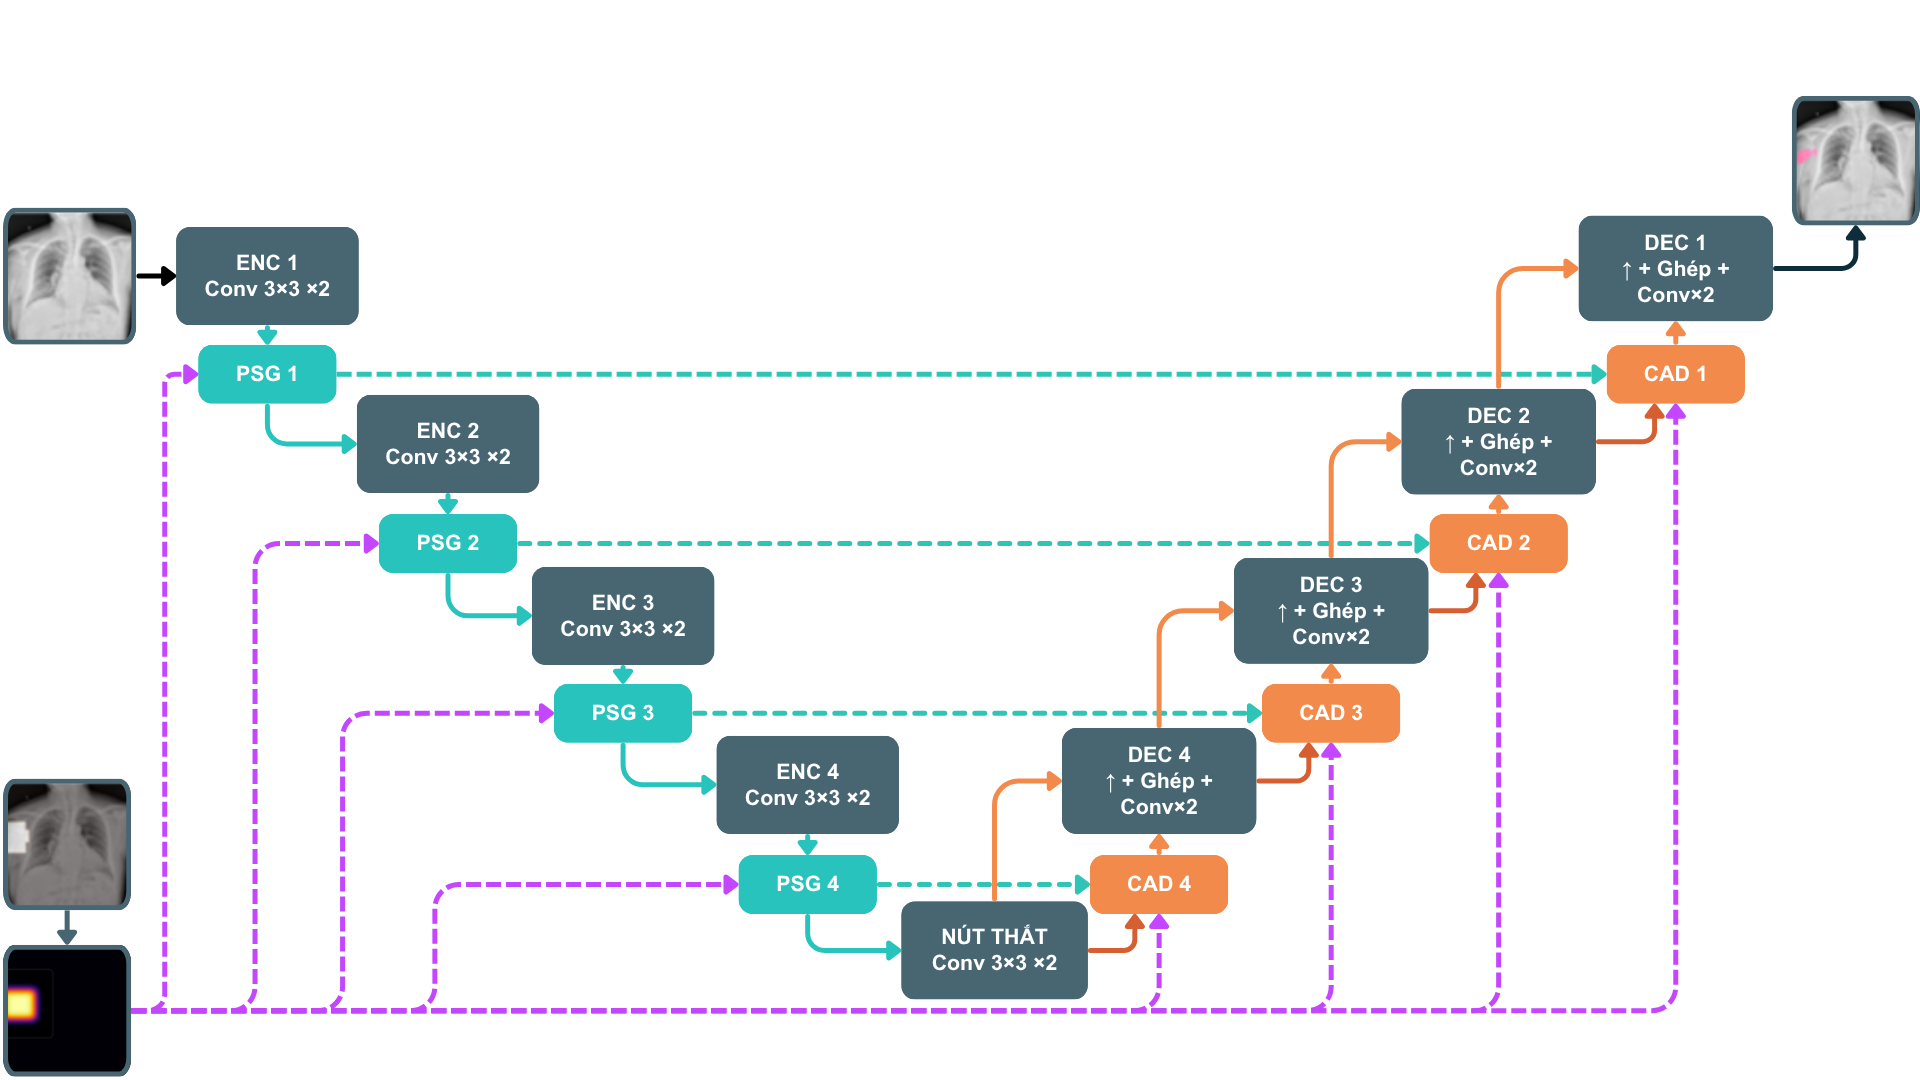
\includegraphics[width=\columnwidth]{images/architecture/architecture_pga_unet.png}
\caption{Overview of PGA-UNet. Prompt information derived from the bounding box is injected into encoder features through PSG and reused in decoder skip attention through CAD.}
\label{fig:arch}
\end{figure}



\section{Experimental Setup}
\label{sec:experimental-setup}
\subsection{Datasets}
We run our experiments on two public bone X-ray datasets. BTXRD is a primary bone tumor dataset with polygon annotations supporting classification, localization, and segmentation \cite{b7}. FracAtlas is a fracture dataset with the same label types \cite{b8}; we convert its segmentation annotations to the same polygon format used for BTXRD before use, and the conversion is released with the reproducibility package. Both datasets are split at the image level, so that every polygon belonging to the same image always falls in the same split (Table~\ref{tab:splits}).

\begin{table}[t]
\caption{Image-level train / validation / test splits. Each lesion polygon is one promptable sample.}
\label{tab:splits}
\centering
\scriptsize
\resizebox{\columnwidth}{!}{%
\begin{tabular}{lcccccc}
\toprule
& \multicolumn{3}{c}{Images} & \multicolumn{3}{c}{Lesion polygons} \\
\cmidrule(lr){2-4}\cmidrule(lr){5-7}
Dataset & Train & Val & Test & Train & Val & Test \\
\midrule
BTXRD & 1{,}493 & 187 & 187 & 1{,}848 & 238 & 232 \\
FracAtlas & 573 & 72 & 72 & 730 & 95 & 92 \\
\bottomrule
\end{tabular}
}
\end{table}

Table~\ref{tab:splits} contains 917 converted lesion polygons for FracAtlas (730 + 95 + 92), whereas the original FracAtlas release reports 922 fracture instances. These totals have not been reconciled at the annotation-ID level. The reported segmentation results therefore refer to the converted annotation set summarized in Table~\ref{tab:splits}. Because the public metadata do not provide enough information to verify strict patient-level separation, images from the same patient could in principle still fall into different splits; we regard this as a limitation of this evaluation. In image-level evaluation, if an image has multiple lesions, the model is run separately for each box, and the resulting probability maps are merged by a pixelwise maximum before thresholding at 0.5; the ground-truth masks are likewise merged by union.

Input images are resized isotropically to preserve aspect ratio, then padded to a square resolution of $128\times128$, $256\times256$, or $512\times512$, depending on the configuration. Images, masks, and prompt maps all undergo this same geometric preprocessing.

\subsection{Training Details}
\label{sec:training}
All CNN models were implemented in PyTorch and trained on a single NVIDIA Tesla T4 GPU with 16 GB memory. PGA-UNet and Attention U-Net were trained separately for each dataset and each resolution; in other words, this article studies one shared architecture family instantiated as separate models, with separate parameter sets for BTXRD and FracAtlas, rather than training a single joint model on both. We used the AdamW optimizer with learning rate $10^{-4}$ and weight decay $10^{-4}$; the loss was the sum of binary cross-entropy and Dice loss. Because the segmentation targets are often small, we additionally tested training PGA-UNet at $512\times512$ with the Dice term replaced by a size-conditioned Tversky loss, and in a separate run, by a Focal Dice loss, with every other setting held fixed. These two replacements are mutually exclusive and are reported later only as a negative control on the training objective. Batch size was 4, training ran for at most 150 epochs, with early stopping at patience 15. All main and ablation experiments share the same fixed training seed, 22120196, which seeds Python, NumPy, and PyTorch on both CPU and CUDA. The primary model-selection criterion was image-level merged Dice, measured on the validation set under the \texttt{center\_shift} condition.

During training, we applied augmentation consisting of horizontal flipping and random rotation within $\pm15^\circ$. PGA-UNet is trained with \texttt{center\_mixed}: \texttt{center\_shift} is chosen with probability 0.8 and \texttt{center\_zoom} with probability 0.2. Because the prompts are all simulated from labeled lesion regions, this is a prompted-segmentation protocol under controlled conditions; the article should be read accordingly, namely as a study of simulated lesion-covering boxes around user-identified lesions, not as an evaluation of unconstrained lesion detection or of boxes fully drawn by a clinician in real practice.

For the fine-tuned SAM-Med2D comparison, the pretrained image encoder was frozen, with only its lightweight Adapter layers trained further, while the prompt encoder and mask decoder were fully updated on each dataset, under the same split protocol. SAM-Med2D was fine-tuned with box prompts only, using the same center-scaled covering and off-center protocol as PGA-UNet; the point-prompt branch and iterative point refinement were both disabled. This box construction differs from the small random-jitter \texttt{get\_boxes\_from\_mask} sampling used by the original SAM-Med2D authors, which we did not apply here. Both validation during SAM-Med2D fine-tuning and the final test-split evaluation report both prompt conditions separately; batch size was 4, at most 150 epochs, early stopping patience 30, and learning rate $10^{-5}$. This matched protocol reduces differences caused by prompt distribution and resolution, but cannot eliminate differences in model scale, initialization, or optimization.

We additionally ran stability experiments using Monte Carlo cross-validation, that is, repeated random image-level splits, as opposed to strict non-overlapping $k$-fold partitioning. These experiments keep the training seed fixed at 22120196 and vary only the split seed, across the values 1, 2, 3, and 4.

Two details are worth noting when interpreting the evaluation results. First, prompt construction itself does not depend on resolution: the plateau heatmap is built and smoothed with a fixed $31\times31$ Gaussian kernel at the original image resolution, and only then resized and padded down to $128\times128$, $256\times256$, or $512\times512$ together with the image. In other words, the same absolute blur is compressed differently at each target resolution, rather than being parameterized separately for each. Second, the Monte Carlo experiments are only auxiliary stability evidence, not intended to replace the fixed train/validation/test split used throughout the main results tables.

\subsection{Baselines and Metrics}
We compare PGA-UNet against an automatic baseline, Attention U-Net \cite{b4}, and three fine-tuned promptable baselines: SAM-Med2D \cite{b2}, MedSAM \cite{b9}, and ScribblePrompt-UNet \cite{b11}. Attention U-Net is trained without a prompt, to show how hard the task becomes when localization must be fully automatic. Among the promptable baselines, SAM-Med2D is fine-tuned and evaluated at $256\times256$ using the same dataset splits and the same box prompts as PGA-UNet, so PGA-UNet at $256$ against SAM-Med2D at $256$ is the article's resolution-matched prompt comparison. MedSAM and ScribblePrompt-UNet run at their own native resolutions ($1024$ and $128$); Table~\ref{tab:sam-ref} reports these alongside PGA-UNet's own $128$ and $512$ results as configuration-specific reference results, each scored in its own frame, and does not use them to establish a cross-model ranking.

To compare the proposed design with conventional ways of using the same box, we evaluate two additional baselines based on the Attention U-Net backbone, without PGA-UNet's Gaussian-prior heatmap, Prompt Spatial Gate, or Conditional Attention Decoder. The channel baseline receives a binary box mask as an additional input channel, whereas the crop baseline receives the image region defined by the box. Only the crop baseline retains the backbone's original attention-gated skip connections unmodified, since the box only changes what image region enters an otherwise-standard Attention U-Net, so we refer to it as Attention U-Net + prompt crop; the channel baseline instead concatenates the mask at the input and decodes through plain, non-gated skip connections, so it is not attention-gated in the same sense as the automatic Attention U-Net reference, and we name it accordingly, U-Net + binary prompt channel. The full PGA-UNet model uses a Gaussian-smoothed heatmap together with explicit encoder and decoder conditioning. These comparisons therefore concern the complete tested configurations, combining differences in prompt representation, backbone gating, and PGA-UNet's own conditioning mechanism, not any one of these in isolation. Both baselines are trained under the same covering and off-center box protocol as PGA-UNet. The binary-prompt PGA-UNet ablation (Section~\ref{sec:ablation}) provides a comparison using the same binary box representation as the channel baseline, without isolating every architectural component. When comparing models against each other, we use the pasted-back full-frame metric for the prompt-crop baseline, not the diagnostic value measured inside the crop frame.

Every comparison table in this article reports Dice and IoU for region overlap, CBL for localization, and HD95 for boundary distance. Dice and IoU are fairly strongly correlated overlap measures; we place them side by side only for the reader's convenience in cross-checking. On the small-lesion subsets specifically, IoU has a low absolute value and is quite sensitive to a few boundary pixels, so Dice is the primary overlap metric used there. Let $(x_p,y_p)$ be the predicted mask centroid, $(x_g,y_g)$ the ground-truth centroid, and $D_{\mathrm{GT}}$ the diagonal length of the ground-truth bounding box; CBL is defined as follows:
\begin{equation}
\mathrm{CBL}=\max\left(0,1-\frac{\sqrt{(x_p-x_g)^2+(y_p-y_g)^2}}{D_{\mathrm{GT}}}\right).
\end{equation}
HD95 is computed from bidirectional boundary distances. When both masks are empty, HD95 is set to 0; if only one mask is empty, HD95 is set to the input side length $S$ (128, 256, or 512 pixels, depending on the configuration). No sample is discarded from the computation. For comparisons spanning resolutions, we additionally report HD95 in normalized form, $\mathrm{HD95}/(\sqrt{2}\,S)$, since a raw pixel distance cannot be directly compared across the $128$, $256$, and $512$ frames. Some subgroup comparisons mix models trained at $256\times256$ and $512\times512$; in that case, everything is scored together in a shared $512\times512$ frame, with the $256\times256$ predictions upsampled before scoring, so every model is measured against exactly the same ground-truth mask, rather than in its own native frame. Cross-model comparisons used to support the main conclusions are restricted to a shared scoring frame: the conventional prompt baselines and PGA-UNet at $512\times512$ (Table~\ref{tab:robust}), and SAM-Med2D and PGA-UNet at $256\times256$ (Table~\ref{tab:sam}). The lower-area subset comparison with SAM-Med2D (Table~\ref{tab:small-sam}) uses $256\times256$ model inputs and a shared $512\times512$ scoring frame. Other operating configurations, including PGA-UNet's own $128$ and $512$ results and the MedSAM and ScribblePrompt-UNet results, are documented separately in Table~\ref{tab:sam-ref} as configuration-specific reference results, each scored in its own frame (PGA-UNet at $128$ or $512$; MedSAM and ScribblePrompt-UNet at the original image resolution, not at the $128$ or $1024$ frame their own network internally resizes to); their raw HD95 values are shown for completeness but are left unbolded. Dice, IoU, and CBL are dimensionless, but they need not remain unchanged after mask resampling and rasterization: a model run at a lower native resolution discretizes a lesion's boundary into fewer pixels before any of these metrics is computed. Consequently, results scored in different frames are not used to establish a cross-model ranking in this article. Normalizing HD95 changes its distance scale but does not remove differences introduced by prediction and ground-truth resampling.

For the training-free self-assessment score, each lesion prompt yields a score $Q$ together with the true thresholded Dice of its own predicted mask; we report the Pearson and Spearman correlation between the two, separately for the covering and off-center conditions. For the candidate-region shortlist, each test image is sampled with 50 boxes whose side length is uniform in $[0.15,0.55]$ of the frame, each box is scored by $Q$, and the five highest-scoring boxes are kept; each retained box is then scored by coverage, the fraction of ground-truth lesion pixels it contains, and no predicted mask enters this coverage measure. From the same 50-box pool we also compute a random-5 baseline (mean over 2,000 resamples per image, without replacement) and an oracle-5 upper bound (the 5 boxes with the truly highest coverage), to check whether $Q$-ranking adds value over chance. As a negative control, the same 50-box sampling is also run on the lesion-free images of each dataset (1879 for BTXRD, 3366 for FracAtlas); with no lesion present there is no coverage to compute, so we report only the distribution of $Q$.

\subsection{Statistical Analysis}
The main baseline comparisons (Tables~\ref{tab:baseline}, \ref{tab:sam}, \ref{tab:extreme}) report descriptive point estimates on the fixed test splits; no paired uncertainty estimates are reported for these comparisons. The existing ablation analysis (Section~\ref{sec:ablation}) uses paired per-image Dice values with a two-sided sign-flip randomization test and percentile bootstrap confidence intervals, each based on $20{,}000$ resamples, with Holm correction as specified in Table~\ref{tab:ablation-sig}. These results are conditional on the evaluated split and trained checkpoints. Four additional image-level splits (Section~\ref{sec:mccv}) characterize variation in PGA-UNet's own performance while keeping its training seed fixed; they do not estimate variation due to the training seed itself, nor do they establish the stability of differences from competing models. The exploratory self-assessment correlation analysis (Section~\ref{sec:selfassess-results}) retains its own permutation $p$-values and bootstrap $95\%$ intervals for Spearman's $\rho$. All resampling uses the fixed seed 22120196.

\subsection{Scope of Analysis}
This article focuses only on prompt-guided segmentation itself. A lesion-screening classification stage was explored in a separate study and is not part of this article. The self-assessment score and the candidate-region shortlist are treated only as auxiliary analyses, within the same narrow scope already stated in Section~\ref{sec:selfassess}; apart from one negative control on lesion-free images, they are not extended any further here. To keep the article compact, we retain only the subgroup analyses that most directly support the main claim: the role of prompt-guided localization (Section~\ref{sec:extreme}), sensitivity to controlled prompt displacement as defined above (Section~\ref{sec:robust}), and observed results on the images with the lowest total lesion area (Section~\ref{sec:small}, where the subgroup definition and its coverage of each test split are given). It should also be reiterated: partial-coverage boxes, negative boxes, and off-target boxes are outside the scope of this study, so the article's claims do not rely on them.


\section{Results}
\label{sec:results}
Unless stated otherwise, every table reports current-protocol numbers: \texttt{center\_mixed} training with 80\% \texttt{center\_shift} and 20\% \texttt{center\_zoom}, 150 epochs, model selection by image-level merged validation Dice under \texttt{center\_shift}, and image-level merged test evaluation. The two test prompt conditions, covering (\texttt{center\_zoom}) and off-center (\texttt{center\_shift}), are reported separately whenever a table carries both.

\subsection{Main Results Across Datasets and Resolutions}
\label{sec:main}
PGA-UNet was trained from scratch at $128\times128$, $256\times256$, and $512\times512$ on each dataset, giving six models. Table~\ref{tab:resolution} reports them under both prompt conditions.

\begin{table}[t]
\caption{PGA-UNet across resolutions, image-level merged. Dice, IoU, CBL and HD95 (native px and normalized $\mathrm{HD95}/(\sqrt{2}\,S)$) given as covering / off-center.}
\label{tab:resolution}
\centering
\scriptsize
\resizebox{\columnwidth}{!}{%
\begin{tabular}{llccccc}
\toprule
Dataset & Res. & Dice & IoU & HD95$_\mathrm{px}$ & HD95$_n$ & CBL \\
\midrule
\multirow{3}{*}{BTXRD}
& $128$ & 0.714 / 0.717 & 0.572 / 0.577 & 5.8 / 5.3 & 0.032 / 0.029 & 0.859 / 0.857 \\
& $256$ & 0.762 / 0.743 & 0.633 / 0.611 & 10.9 / 12.8 & 0.030 / 0.035 & 0.902 / 0.885 \\
& $512$ & \textbf{0.782} / \textbf{0.774} & \textbf{0.661} / \textbf{0.652} & 22.8 / 24.5 & 0.031 / 0.034 & \textbf{0.918} / \textbf{0.912} \\
\midrule
\multirow{3}{*}{FracAtlas}
& $128$ & 0.596 / 0.542 & 0.445 / 0.389 & 8.1 / 9.5 & 0.044 / 0.053 & 0.849 / 0.790 \\
& $256$ & 0.629 / 0.594 & 0.470 / 0.436 & 10.6 / 11.7 & 0.029 / 0.032 & 0.895 / 0.849 \\
& $512$ & \textbf{0.727} / \textbf{0.713} & \textbf{0.585} / \textbf{0.570} & 10.5 / 10.4 & \textbf{0.015} / \textbf{0.014} & \textbf{0.913} / \textbf{0.897} \\
\bottomrule
\end{tabular}
}
\end{table}

The reported Dice values increase from the $128$ to the $256$ and $512$ configurations on both datasets and under both prompt conditions, with FracAtlas gaining more. Each configuration is scored in its own output frame, so these are operating-configuration results that combine changes in model input resolution and mask sampling; they do not isolate an internal feature-preservation mechanism or provide a common-frame estimate of the effect of input resolution alone. Because HD95 in raw pixels cannot be compared across differently sized frames, we also report the normalized form: it stays near $0.03$ across the BTXRD resolutions and decreases on FracAtlas as the frame grows. Note that each model is evaluated only on the dataset it was trained on; the article makes no claim about cross-dataset transfer.

\subsection{Comparison Against Automatic and Prompt-Matched Baselines}
\label{sec:baseline}
With no support at all in finding the lesion, Attention U-Net reaches only 0.517 Dice on BTXRD and 0.342 on FracAtlas at $512\times512$, with HD95 exceeding 120 pixels on both datasets (Table~\ref{tab:baseline}). The no-prompt reference addresses a different input setting than every other row in this table, and is not used to attribute the differences below to the proposed architecture.

Under covering prompts at $512\times512$, PGA-UNet obtains Dice scores of 0.782 on BTXRD and 0.727 on FracAtlas, compared with 0.760 and 0.593 for the binary prompt-channel baseline and 0.741 and 0.590 for the prompt-crop baseline (Table~\ref{tab:baseline}). An additional comparison is available from the binary-prompt PGA-UNet ablation (Table~\ref{tab:ablation}): it obtains 0.788 and 0.668 respectively, using the same binary box representation as the channel baseline. This provides descriptive support for the explicit conditioning design beyond a change to Gaussian prompt encoding. These baselines control access to the box location, but the full PGA-UNet model also differs in prompt representation from the channel and crop baselines, so the comparisons here do not separately identify the effects of every architectural component, and no paired uncertainty estimates are reported for these baseline differences.

\begin{table}[t]
\caption{Comparison at $512\times512$ under covering prompts. Attention U-Net (no prompt) receives no box; the other rows use the same box PGA-UNet receives. The Delta Dice column is each row minus PGA-UNet.}
\label{tab:baseline}
\centering
\scriptsize
\resizebox{\columnwidth}{!}{%
\begin{tabular}{llccccc}
\toprule
Dataset & Model & Dice & $\Delta$Dice & IoU & HD95 & CBL \\
\midrule
\multirow{4}{*}{BTXRD}
& Attention U-Net (no prompt) & 0.517 & $-0.265$ & 0.418 & 120.4 & 0.620 \\
& U-Net + binary prompt channel & 0.760 & $-0.022$ & 0.635 & 33.0 & 0.895 \\
& Attention U-Net + prompt crop & 0.741 & $-0.041$ & 0.615 & 24.7 & 0.912 \\
& PGA-UNet & \textbf{0.782} & --- & \textbf{0.661} & \textbf{22.8} & \textbf{0.918} \\
\midrule
\multirow{4}{*}{FracAtlas}
& Attention U-Net (no prompt) & 0.342 & $-0.385$ & 0.253 & 139.9 & 0.478 \\
& U-Net + binary prompt channel & 0.593 & $-0.134$ & 0.434 & 22.9 & 0.887 \\
& Attention U-Net + prompt crop & 0.590 & $-0.137$ & 0.451 & 22.0 & 0.865 \\
& PGA-UNet & \textbf{0.727} & --- & \textbf{0.585} & \textbf{10.5} & \textbf{0.913} \\
\bottomrule
\end{tabular}
}
\end{table}

In the reported point estimates, the differences between the no-prompt and conventional prompted configurations are larger than the differences among the prompted configurations. The latter comparisons, between PGA-UNet and the two conventional prompt baselines, provide the more specific evidence for the proposed conditioning design.

\subsection{Attention U-Net Top-Dice and Bottom-Dice Subsets}
\label{sec:extreme}
To probe the same comparison on a different split of the test images, we ranked them by Attention U-Net Dice, kept the top 50 and bottom 50 per dataset, and re-ran all four models on those exact images (Table~\ref{tab:extreme}, covering prompts). On the BTXRD top-50 subset, the three prompted configurations have Dice values between 0.844 and 0.862. On the FracAtlas top-50 subset, their values span a wider range, from 0.605 to 0.754. On the bottom-50, Attention U-Net's Dice is far lower, down to 0.031 on BTXRD and 0.169 on FracAtlas, while PGA-UNet's is 0.712 and 0.687, and PGA-UNet leads the two conventional prompt baselines by 0.04 to 0.07 Dice on BTXRD and by 0.10 to 0.19 on FracAtlas within this group.

These subsets describe the selected images and are not independent evidence that the proposed method preferentially benefits intrinsically difficult cases: the Attention U-Net top- and bottom-Dice groups are defined entirely by that same baseline's own predictions, not by any external difficulty criterion, and on FracAtlas, whose test split has only 72 images (Table~\ref{tab:splits}), the two groups are not independent samples: by construction at least $50+50-72=28$ images must belong to both, so the two rows are less a comparison between two disjoint image sets than a comparison between the 22 images each group excludes; on BTXRD, with 187 test images, the two groups share no images. We report the FracAtlas split as computed, but this overlap should be kept in mind when reading its top-50/bottom-50 gap.

\begin{table}[t]
\caption{Top-Dice and bottom-Dice subsets at $512\times512$, 50 images per group, covering prompts. Groups are defined by plain Attention U-Net.}
\label{tab:extreme}
\centering
\scriptsize
\resizebox{\columnwidth}{!}{%
\begin{tabular}{lllcccc}
\toprule
Dataset & Group & Model & Dice & IoU & HD95 & CBL \\
\midrule
\multirow{8}{*}{BTXRD}
& \multirow{4}{*}{Top-50}
  & Attention U-Net & 0.872 & 0.775 & 35.0 & 0.945 \\
& & U-Net + channel & 0.846 & 0.740 & 24.3 & 0.942 \\
& & AttUNet + crop & 0.844 & 0.739 & 27.5 & 0.946 \\
& & PGA-UNet & 0.862 & 0.763 & 19.2 & 0.944 \\
\cmidrule(l){2-7}
& \multirow{4}{*}{Bottom-50}
  & Attention U-Net & 0.031 & 0.016 & 277.8 & 0.105 \\
& & U-Net + channel & 0.668 & 0.541 & 43.3 & 0.831 \\
& & AttUNet + crop & 0.652 & 0.518 & 17.6 & 0.875 \\
& & PGA-UNet & \textbf{0.712} & \textbf{0.589} & 23.2 & \textbf{0.879} \\
\midrule
\multirow{8}{*}{FracAtlas}
& \multirow{4}{*}{Top-50}
  & Attention U-Net & 0.493 & 0.365 & 85.7 & 0.640 \\
& & U-Net + channel & 0.605 & 0.447 & 26.6 & 0.887 \\
& & AttUNet + crop & 0.658 & 0.515 & 24.9 & 0.881 \\
& & PGA-UNet & \textbf{0.754} & \textbf{0.615} & 10.6 & \textbf{0.927} \\
\cmidrule(l){2-7}
& \multirow{4}{*}{Bottom-50}
  & Attention U-Net & 0.169 & 0.106 & 182.3 & 0.315 \\
& & U-Net + channel & 0.574 & 0.416 & 25.3 & 0.875 \\
& & AttUNet + crop & 0.509 & 0.369 & 26.0 & 0.834 \\
& & PGA-UNet & \textbf{0.687} & \textbf{0.535} & 11.8 & \textbf{0.896} \\
\bottomrule
\end{tabular}
}
\end{table}

\begin{figure}[t]
\centering
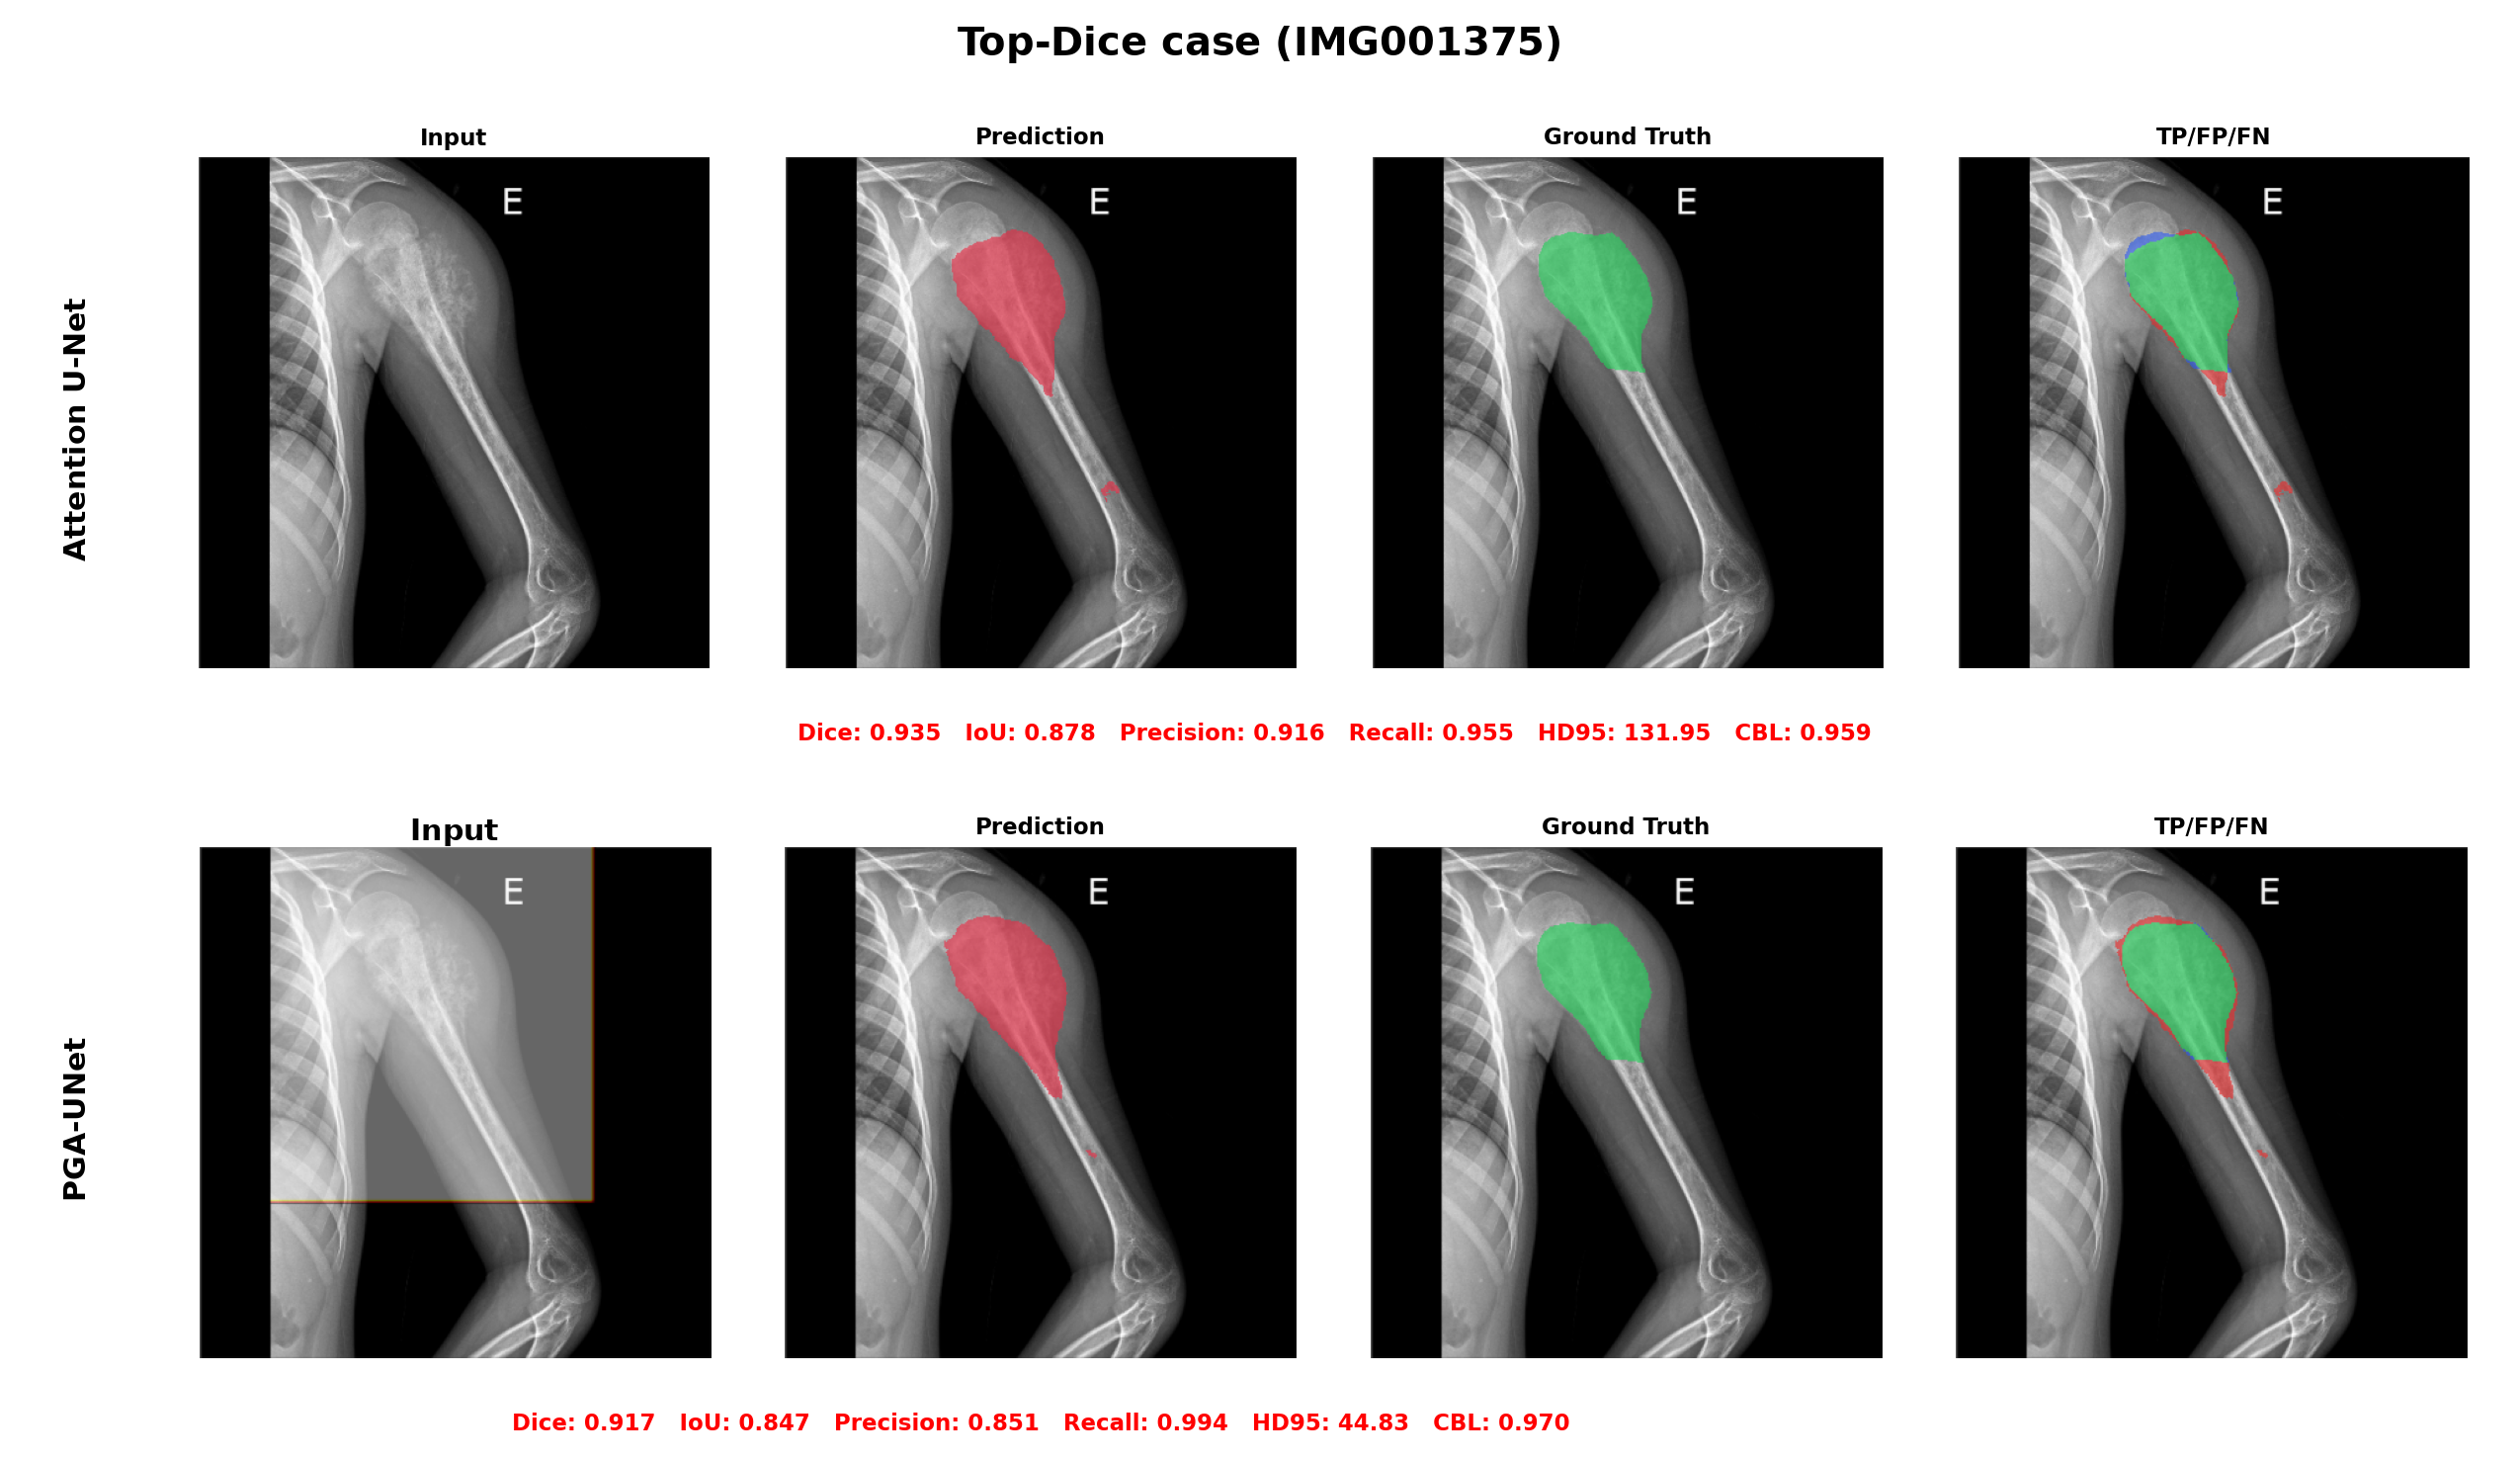
\includegraphics[width=\columnwidth]{images/results/unet_extreme_groups_btxrd_top.png}
\caption{Attention U-Net (no prompt) vs PGA-UNet on BTXRD, Attention U-Net top-Dice case (IMG001375). Both models do well on an easy case.}
\label{fig:extreme-btxrd-top}
\end{figure}

\begin{figure}[t]
\centering
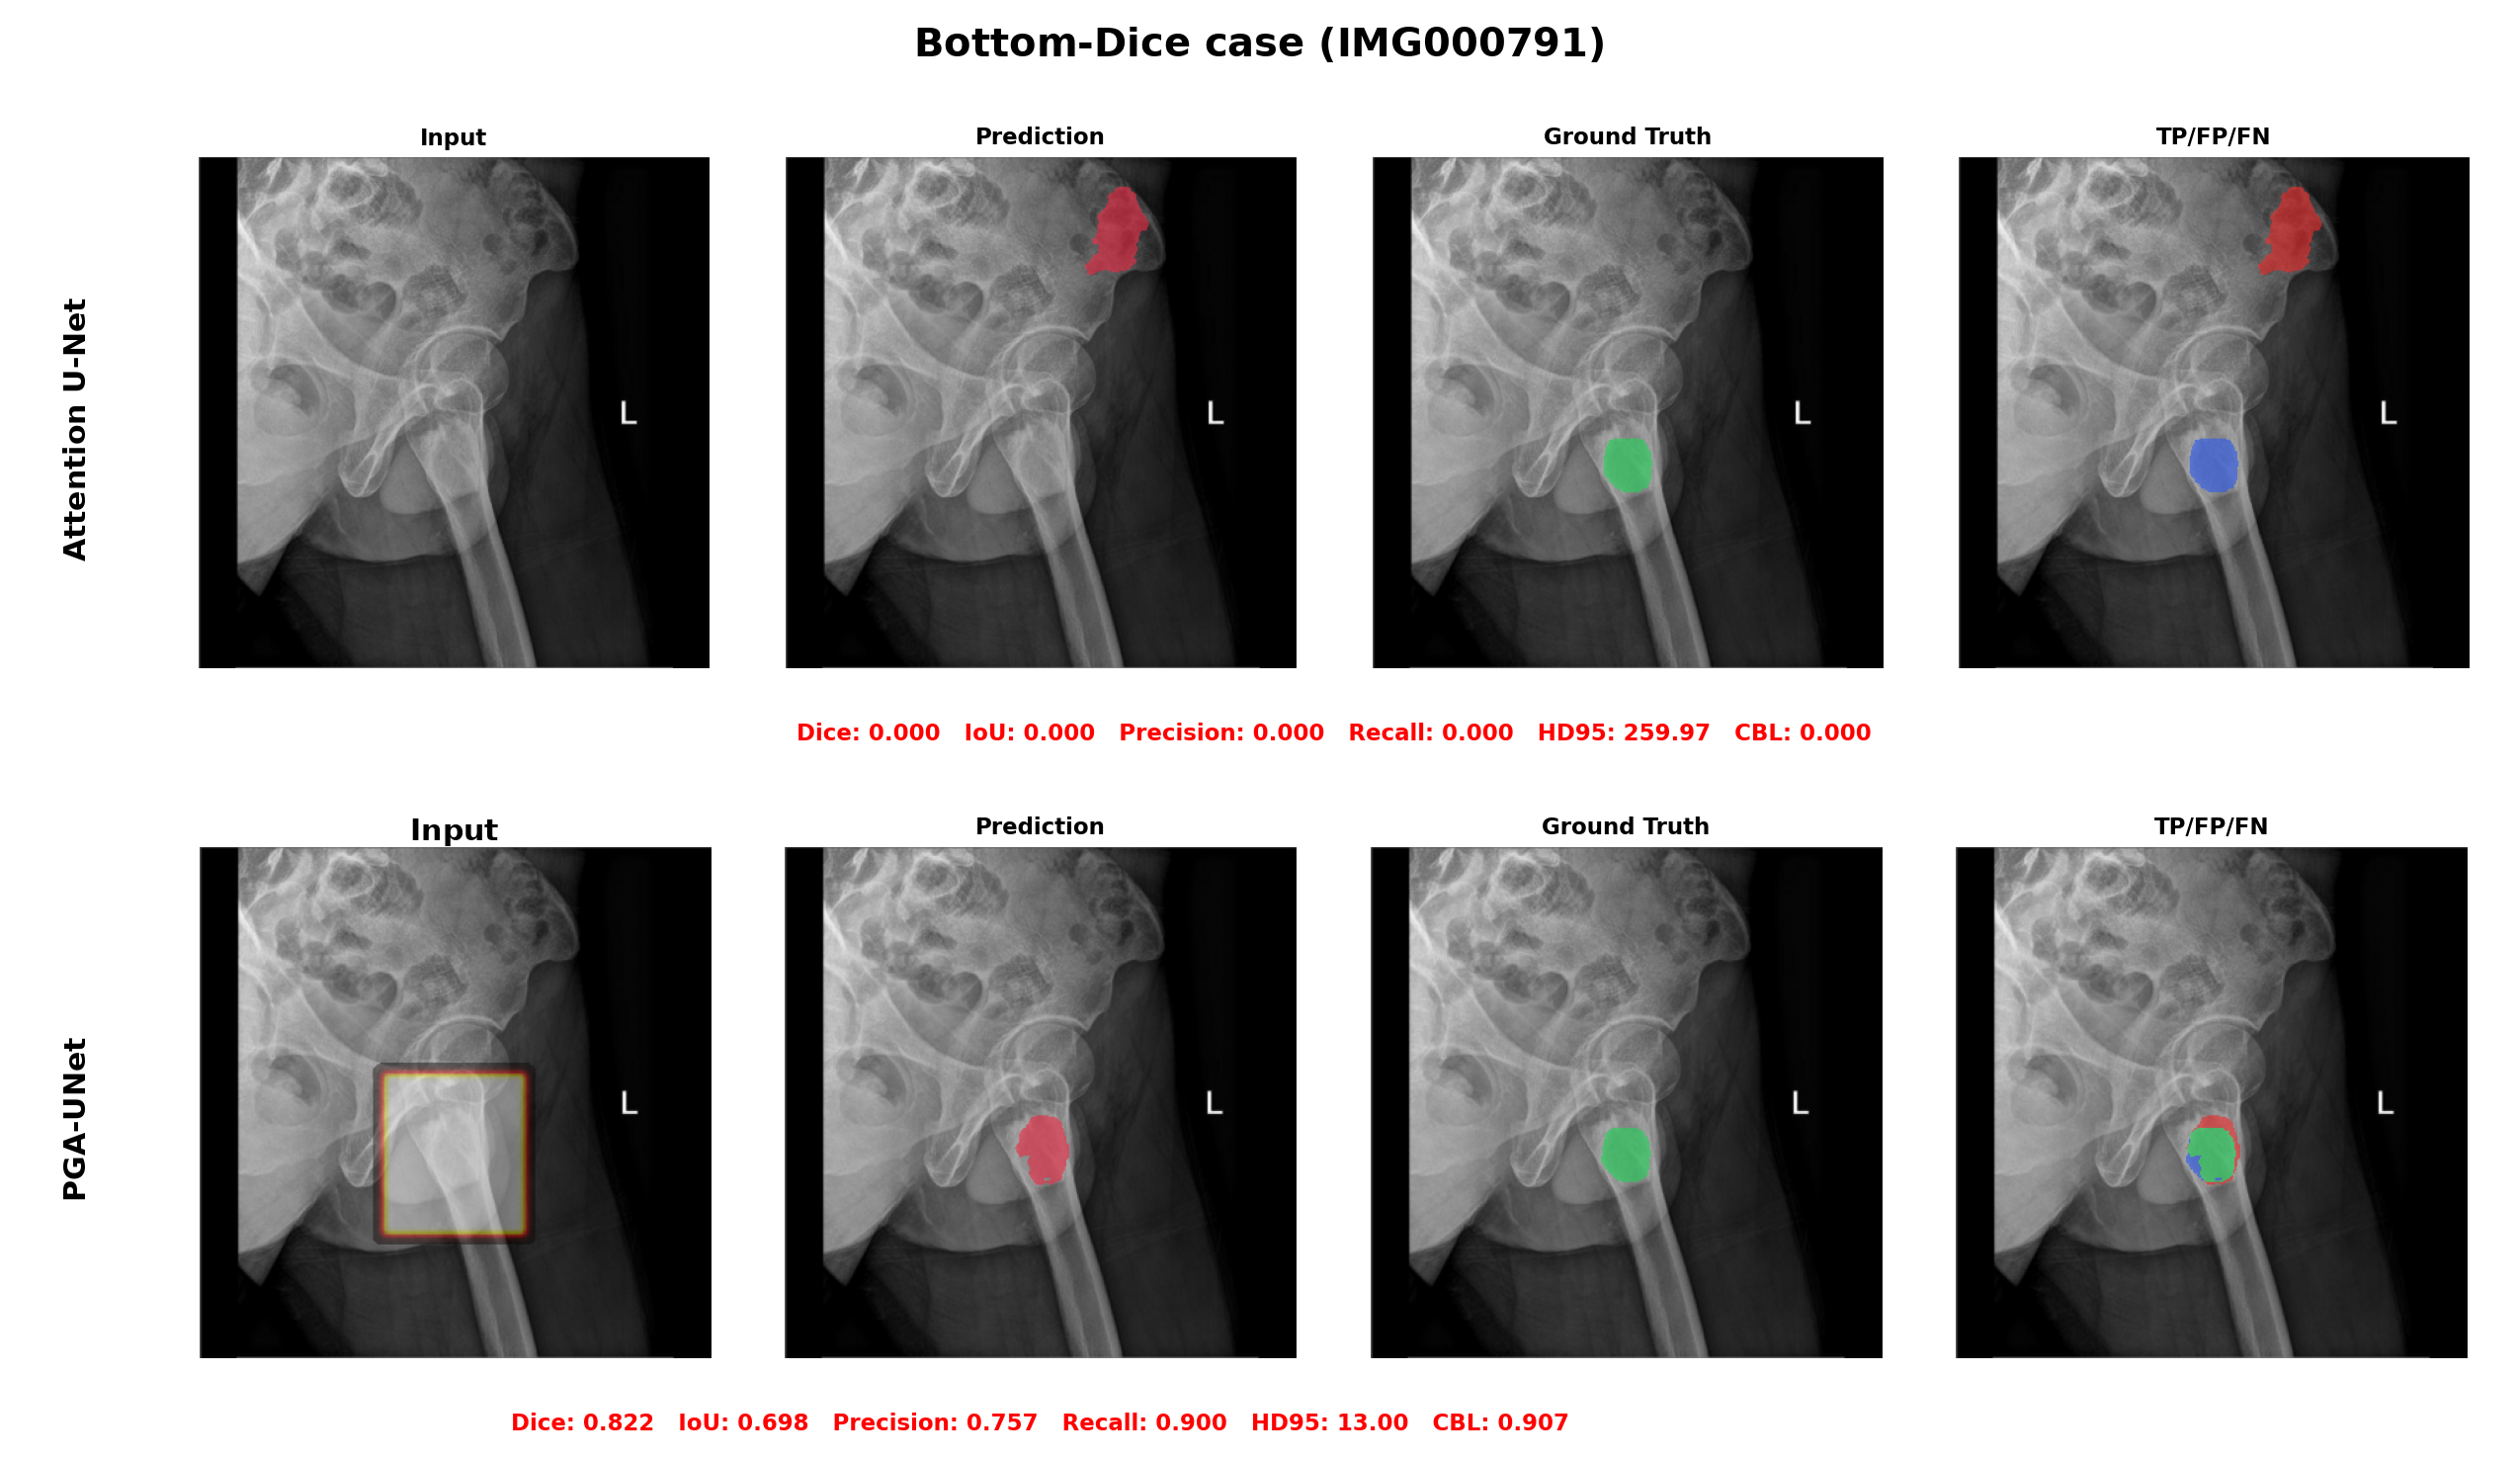
\includegraphics[width=\columnwidth]{images/results/unet_extreme_groups_btxrd_bottom.png}
\caption{Attention U-Net (no prompt) vs PGA-UNet on BTXRD, Attention U-Net bottom-Dice case (IMG000791). Without a prompt, Attention U-Net's prediction is badly mislocated; the prompt-conditioned PGA-UNet still recovers the lesion.}
\label{fig:extreme-btxrd-bottom}
\end{figure}

\subsection{Comparison Against Promptable Baselines}
\label{sec:sam}
The evaluated promptable references are SAM-Med2D, MedSAM, and ScribblePrompt-UNet. Tables~\ref{tab:sam} and \ref{tab:sam-ref} report their zero-shot and fine-tuned results under the specified box-prompt protocol. Within each evaluated model configuration, fine-tuning yields higher observed Dice than zero-shot initialization on both datasets. Comparisons used to support the main conclusions are restricted to the shared scoring frames described below.

At a shared input and scoring resolution of $256\times256$, PGA-UNet obtains Dice scores of 0.762 and 0.629 on BTXRD and FracAtlas, compared with 0.630 and 0.563 for the evaluated fine-tuned SAM-Med2D configuration (Table~\ref{tab:sam}). The boundary results are mixed: PGA-UNet has lower HD95 on BTXRD (10.9 vs 17.3), whereas SAM-Med2D has lower HD95 on FracAtlas (8.0 vs 10.6). These fixed-split results concern the tested configurations and do not establish a general ranking of CNN and foundation-model architectures.

\begin{table}[t]
\caption{Comparison with SAM-Med2D using $256\times256$ model inputs and a shared $256\times256$ scoring frame, under covering prompts, image-level merged. Values are descriptive point estimates; shared resolution and prompts do not equate the models' pretraining or optimization procedures.}
\label{tab:sam}
\centering
\scriptsize
\resizebox{\columnwidth}{!}{%
\begin{tabular}{llcccc}
\toprule
Dataset & Model & Dice & IoU & HD95 & CBL \\
\midrule
\multirow{3}{*}{BTXRD}
& SAM-Med2D zero-shot  & 0.255 & 0.156 & 41.2  & 0.734 \\
& SAM-Med2D fine-tuned & 0.630 & 0.497 & 17.3  & 0.836 \\
& PGA-UNet $256$ & \textbf{0.762} & \textbf{0.633} & \textbf{10.9} & \textbf{0.902} \\
\midrule
\multirow{3}{*}{FracAtlas}
& SAM-Med2D zero-shot  & 0.262 & 0.156 & \textbf{21.3}  & 0.752 \\
& SAM-Med2D fine-tuned & 0.563 & 0.417 & \textbf{8.0}  & 0.846 \\
& PGA-UNet $256$ & \textbf{0.629} & \textbf{0.470} & 10.6 & \textbf{0.895} \\
\bottomrule
\end{tabular}
}
\end{table}

The MedSAM and ScribblePrompt-UNet results, together with PGA-UNet's own $128$ and $512$ configurations, are retained as configuration-specific reference results in Table~\ref{tab:sam-ref} because their scoring frames differ from the shared $256\times256$ frame used above; each is scored in its own frame, network input and scoring frame are reported separately, and these numbers are not used to establish a cross-model ranking. The change from covering to off-center prompts is discussed separately in Section~\ref{sec:robust}.

\begin{table}[t]
\caption{Configuration-specific reference results under covering prompts, image-level merged. Network input resolution and metric scoring frame are reported separately. Scores from different frames are retained to document the evaluated configurations and are not used to establish a cross-model ranking; raw HD95 values from different scoring frames are not directly comparable and are left unbolded throughout.}
\label{tab:sam-ref}
\centering
\scriptsize
\resizebox{\columnwidth}{!}{%
\begin{tabular}{llccccc}
\toprule
Dataset & Model & Input / frame & Dice & IoU & HD95 & CBL \\
\midrule
\multirow{6}{*}{BTXRD}
& PGA-UNet             & 512 / 512  & 0.782 & 0.661 & 22.8 & 0.918 \\
& PGA-UNet             & 128 / 128  & 0.714 & 0.572 & 5.8 & 0.859 \\
& MedSAM zero-shot     & 1024 / orig. & 0.304 & 0.185 & 242.4 & 0.832 \\
& MedSAM fine-tuned    & 1024 / orig. & 0.724 & 0.590 & 79.9  & 0.883 \\
& ScribblePrompt zero-shot  & 128 / orig. & 0.411 & 0.285 & 232.2 & 0.774 \\
& ScribblePrompt fine-tuned & 128 / orig. & 0.653 & 0.514 & 122.7 & 0.853 \\
\midrule
\multirow{6}{*}{FracAtlas}
& PGA-UNet             & 512 / 512  & 0.727 & 0.585 & 10.5 & 0.913 \\
& PGA-UNet             & 128 / 128  & 0.596 & 0.445 & 8.1 & 0.849 \\
& MedSAM zero-shot     & 1024 / orig. & 0.319 & 0.193 & 60.1 & 0.843 \\
& MedSAM fine-tuned    & 1024 / orig. & 0.729 & 0.583 & 16.2 & 0.900 \\
& ScribblePrompt zero-shot  & 128 / orig. & 0.432 & 0.290 & 34.2 & 0.832 \\
& ScribblePrompt fine-tuned & 128 / orig. & 0.679 & 0.527 & 17.9 & 0.891 \\
\bottomrule
\end{tabular}
}
\end{table}

\subsection{Descriptive Analysis of Images with Lower Total Lesion Area}
\label{sec:small}
The lower-lesion-area image subset contains the 50 test images per dataset with the smallest total merged lesion-mask area in the common reference frame, ranging from 7 to 433 pixels on BTXRD and 145 to 944 pixels on FracAtlas. This image-level definition covers 26.7\% of BTXRD's test images and 69.4\% of FracAtlas's (Table~\ref{tab:splits}) and does not measure per-lesion sensitivity or represent matched area quantiles across the two datasets. Combined with the Attention U-Net top- and bottom-Dice subsets of Section~\ref{sec:extreme}, which are defined by that baseline's own predictions rather than an external difficulty criterion, these analyses describe the selected images and are not independent evidence that the proposed method preferentially benefits small lesions or intrinsically difficult cases in general.

Tables~\ref{tab:small-sam} and \ref{tab:small-att} use a shared $512\times512$ scoring frame, whereas Table~\ref{tab:small-res} reports results scored in each configuration's own frame. The $256$-input results in Table~\ref{tab:small-sam} therefore differ from the corresponding $256$-frame results in Table~\ref{tab:small-res}, even though both use the same 50-image subset. This is a separate distinction from the fact that Table~\ref{tab:resolution} additionally evaluates a different image set, the full test split rather than this 50-image subset, so its numbers are not compared here as though frame were the only difference.

\paragraph{Against SAM-Med2D at the matched resolution}
SAM-Med2D struggles clearly at this lesion size (Table~\ref{tab:small-sam}). Even after fine-tuning at $256$, it reaches only 0.256 Dice on BTXRD and 0.371 on FracAtlas; in zero-shot mode it reaches 0.139 and 0.205. PGA-UNet at the same $256$ resolution still holds 0.705 and 0.648, with far lower HD95.

\begin{table}[t]
\caption{Small-lesion subset, PGA-UNet vs SAM-Med2D at the matched $256\times256$ resolution. 50 images per dataset, covering prompts, scored in a shared $512\times512$ frame.}
\label{tab:small-sam}
\centering
\scriptsize
\resizebox{\columnwidth}{!}{%
\begin{tabular}{llcccc}
\toprule
Dataset & Model & Dice & IoU & HD95 & CBL \\
\midrule
\multirow{3}{*}{BTXRD}
& SAM-Med2D zero-shot $256$ & 0.139 & 0.082 & 62.4 & 0.515 \\
& SAM-Med2D fine-tuned $256$ & 0.256 & 0.170 & 123.8 & 0.561 \\
& PGA-UNet $256$ & \textbf{0.705} & \textbf{0.559} & \textbf{14.7} & \textbf{0.877} \\
\midrule
\multirow{3}{*}{FracAtlas}
& SAM-Med2D zero-shot $256$ & 0.205 & 0.123 & 33.5 & 0.659 \\
& SAM-Med2D fine-tuned $256$ & 0.371 & 0.256 & 62.1 & 0.736 \\
& PGA-UNet $256$ & \textbf{0.648} & \textbf{0.491} & \textbf{20.6} & \textbf{0.897} \\
\bottomrule
\end{tabular}
}
\end{table}

\begin{figure}[t]
\centering
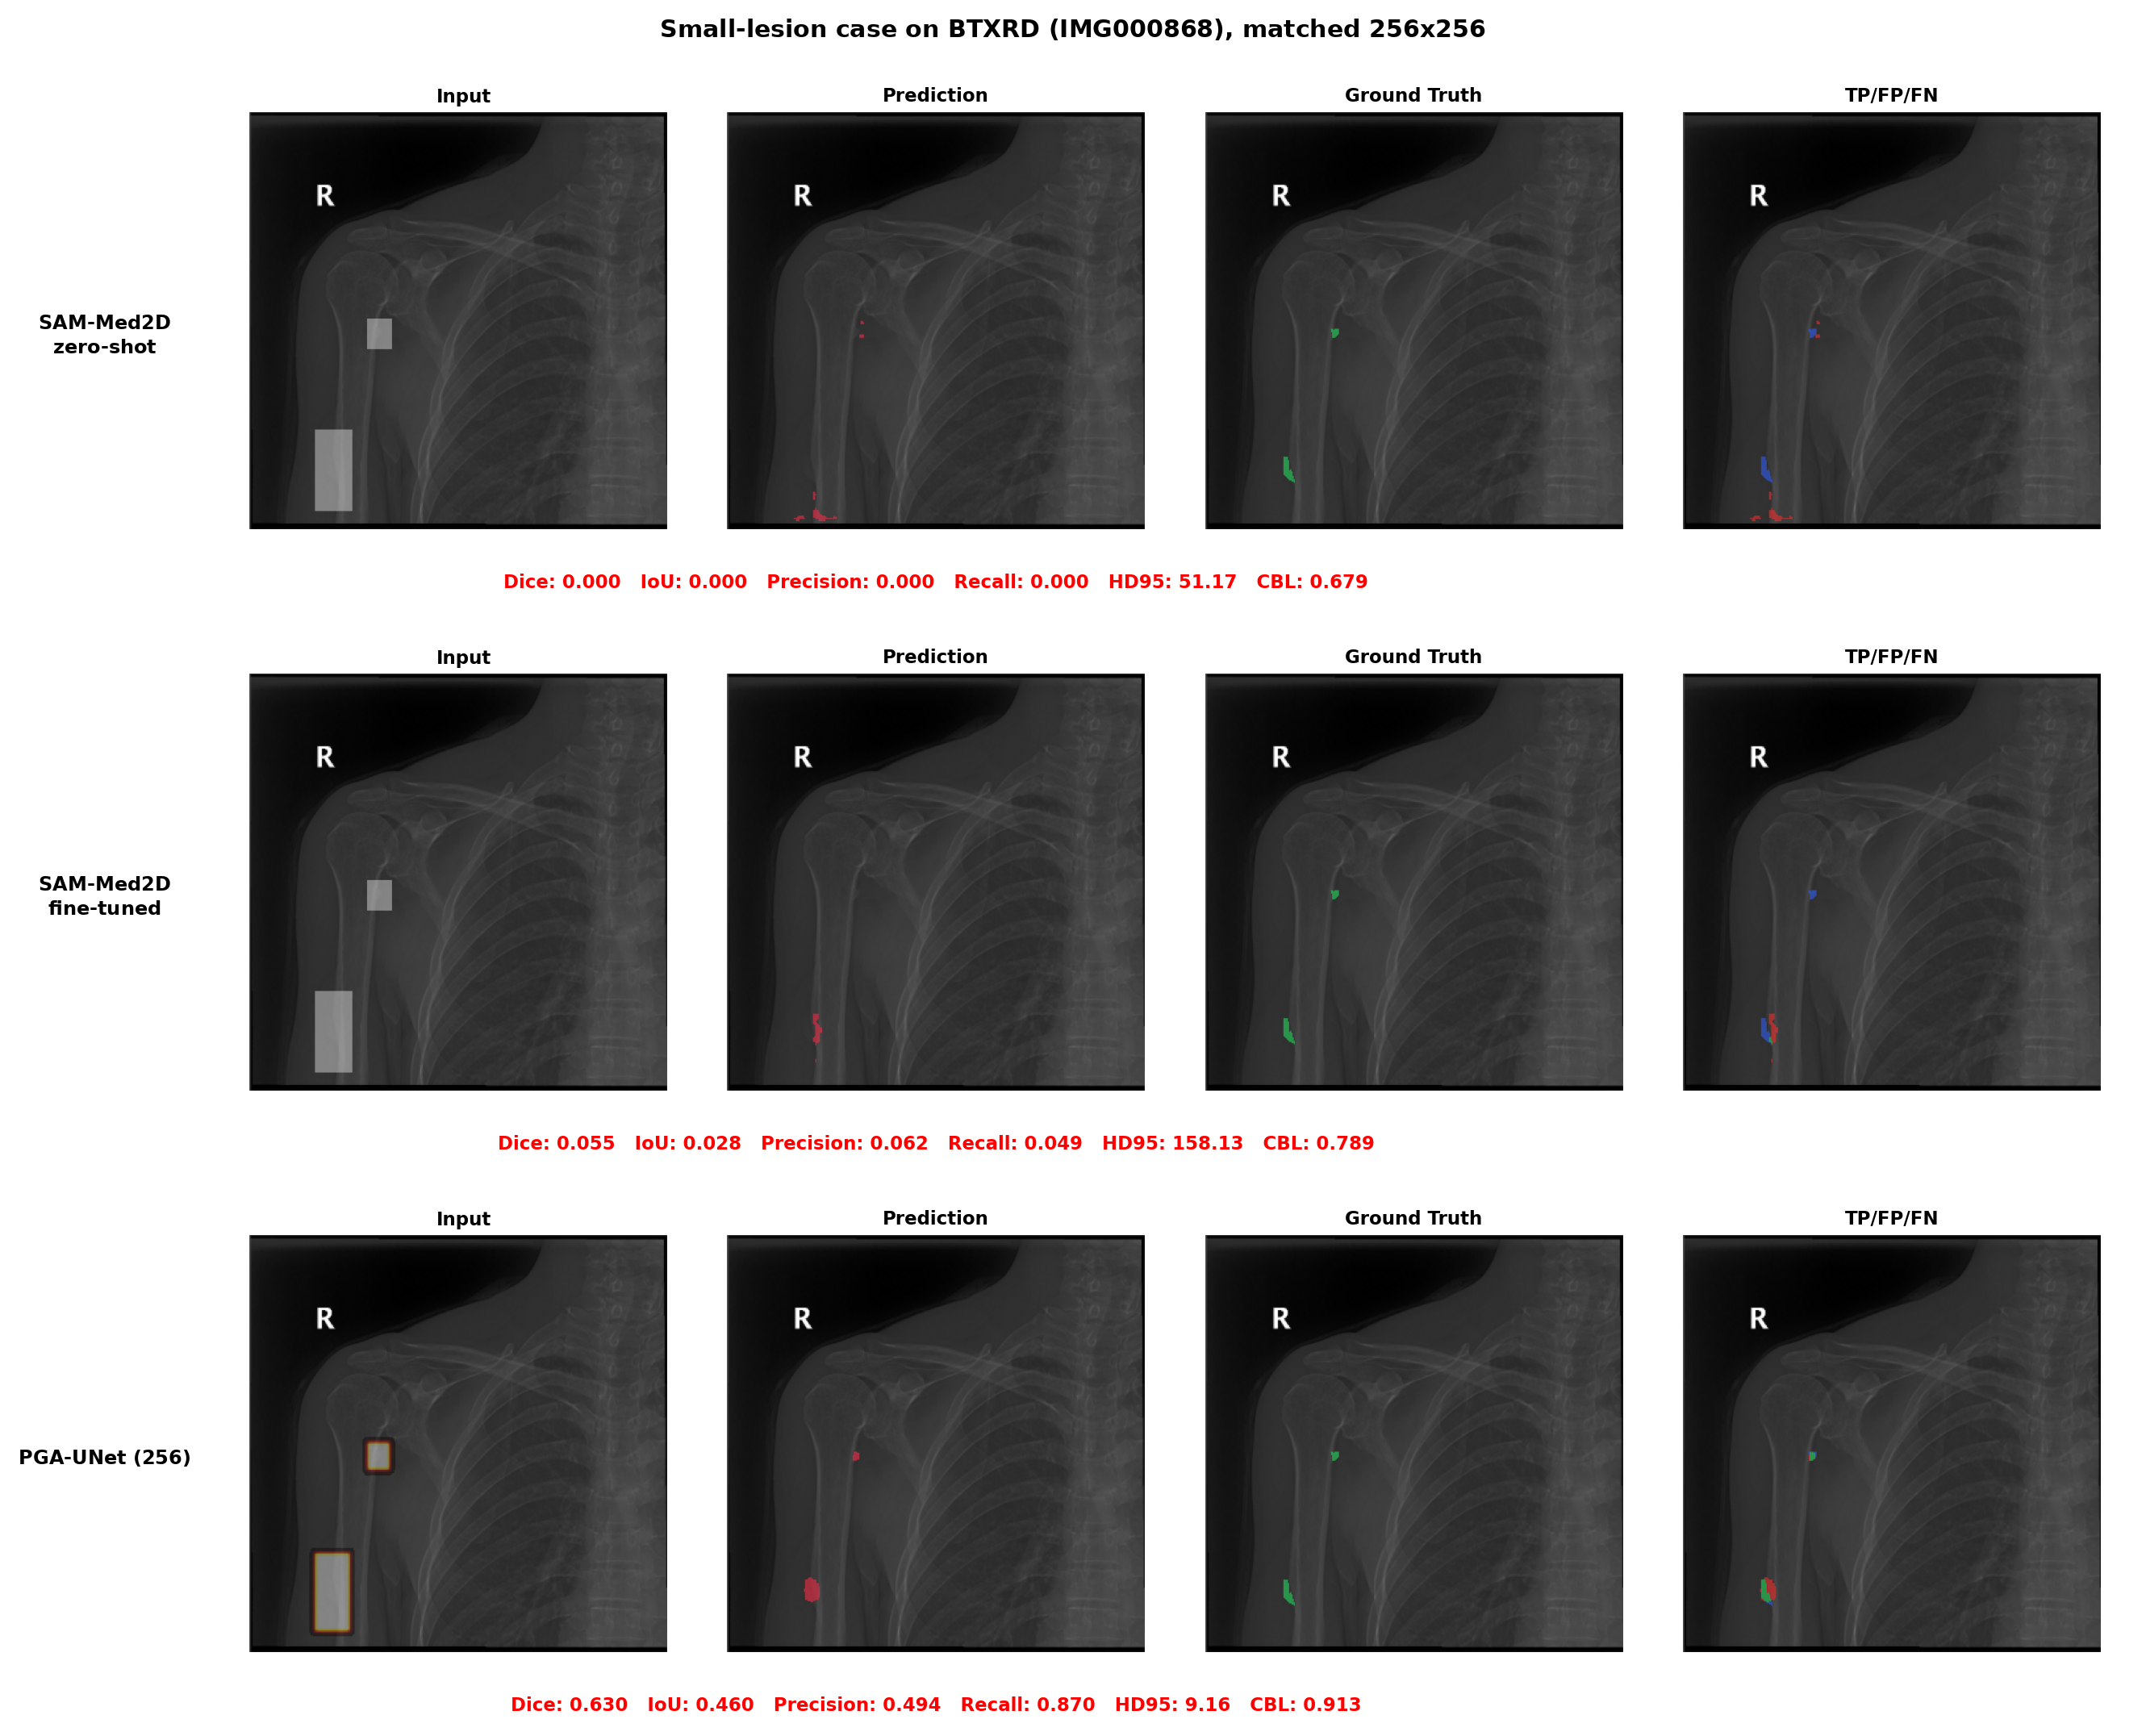
\includegraphics[width=\columnwidth]{images/results/small_lesion_sam_pga256.png}
\caption{Small-lesion case on BTXRD (IMG000868, two GT polygons): SAM-Med2D zero-shot, SAM-Med2D fine-tuned, and PGA-UNet, all at $256\times256$. Both SAM-Med2D variants miss the lesions almost entirely (Dice 0.000, 0.055); PGA-UNet reaches 0.630.}
\label{fig:small-sam}
\end{figure}

\paragraph{Against prompt-matched conventional baselines at $512$}
Given the same box at $512$, the two conventional prompt baselines trail PGA-UNet by about 0.04 on BTXRD and by 0.11 to 0.16 on FracAtlas, while prompt-free Attention U-Net drops to only about 0.28 (Table~\ref{tab:small-att}). The prompt-crop variant reaches a lower HD95 on BTXRD, perhaps because its tight crop suits a compact target well, but this does not carry over to FracAtlas.

\begin{table}[t]
\caption{Small-lesion subset at $512\times512$, PGA-UNet vs the two conventional prompt baselines. 50 images per dataset, covering prompts.}
\label{tab:small-att}
\centering
\scriptsize
\resizebox{\columnwidth}{!}{%
\begin{tabular}{llcccc}
\toprule
Dataset & Model & Dice & IoU & HD95 & CBL \\
\midrule
\multirow{4}{*}{BTXRD}
& Attention U-Net (no prompt) & 0.283 & 0.219 & 178.2 & 0.283 \\
& U-Net + binary prompt channel & 0.728 & 0.591 & 14.2 & 0.879 \\
& Attention U-Net + prompt crop & 0.724 & 0.602 & \textbf{5.5} & \textbf{0.909} \\
& PGA-UNet & \textbf{0.766} & \textbf{0.637} & 14.0 & 0.897 \\
\midrule
\multirow{4}{*}{FracAtlas}
& Attention U-Net (no prompt) & 0.291 & 0.216 & 139.4 & 0.401 \\
& U-Net + binary prompt channel & 0.610 & 0.449 & 21.9 & 0.888 \\
& Attention U-Net + prompt crop & 0.564 & 0.425 & 22.6 & 0.855 \\
& PGA-UNet & \textbf{0.720} & \textbf{0.578} & \textbf{8.3} & \textbf{0.907} \\
\bottomrule
\end{tabular}
}
\end{table}

\begin{figure}[t]
\centering
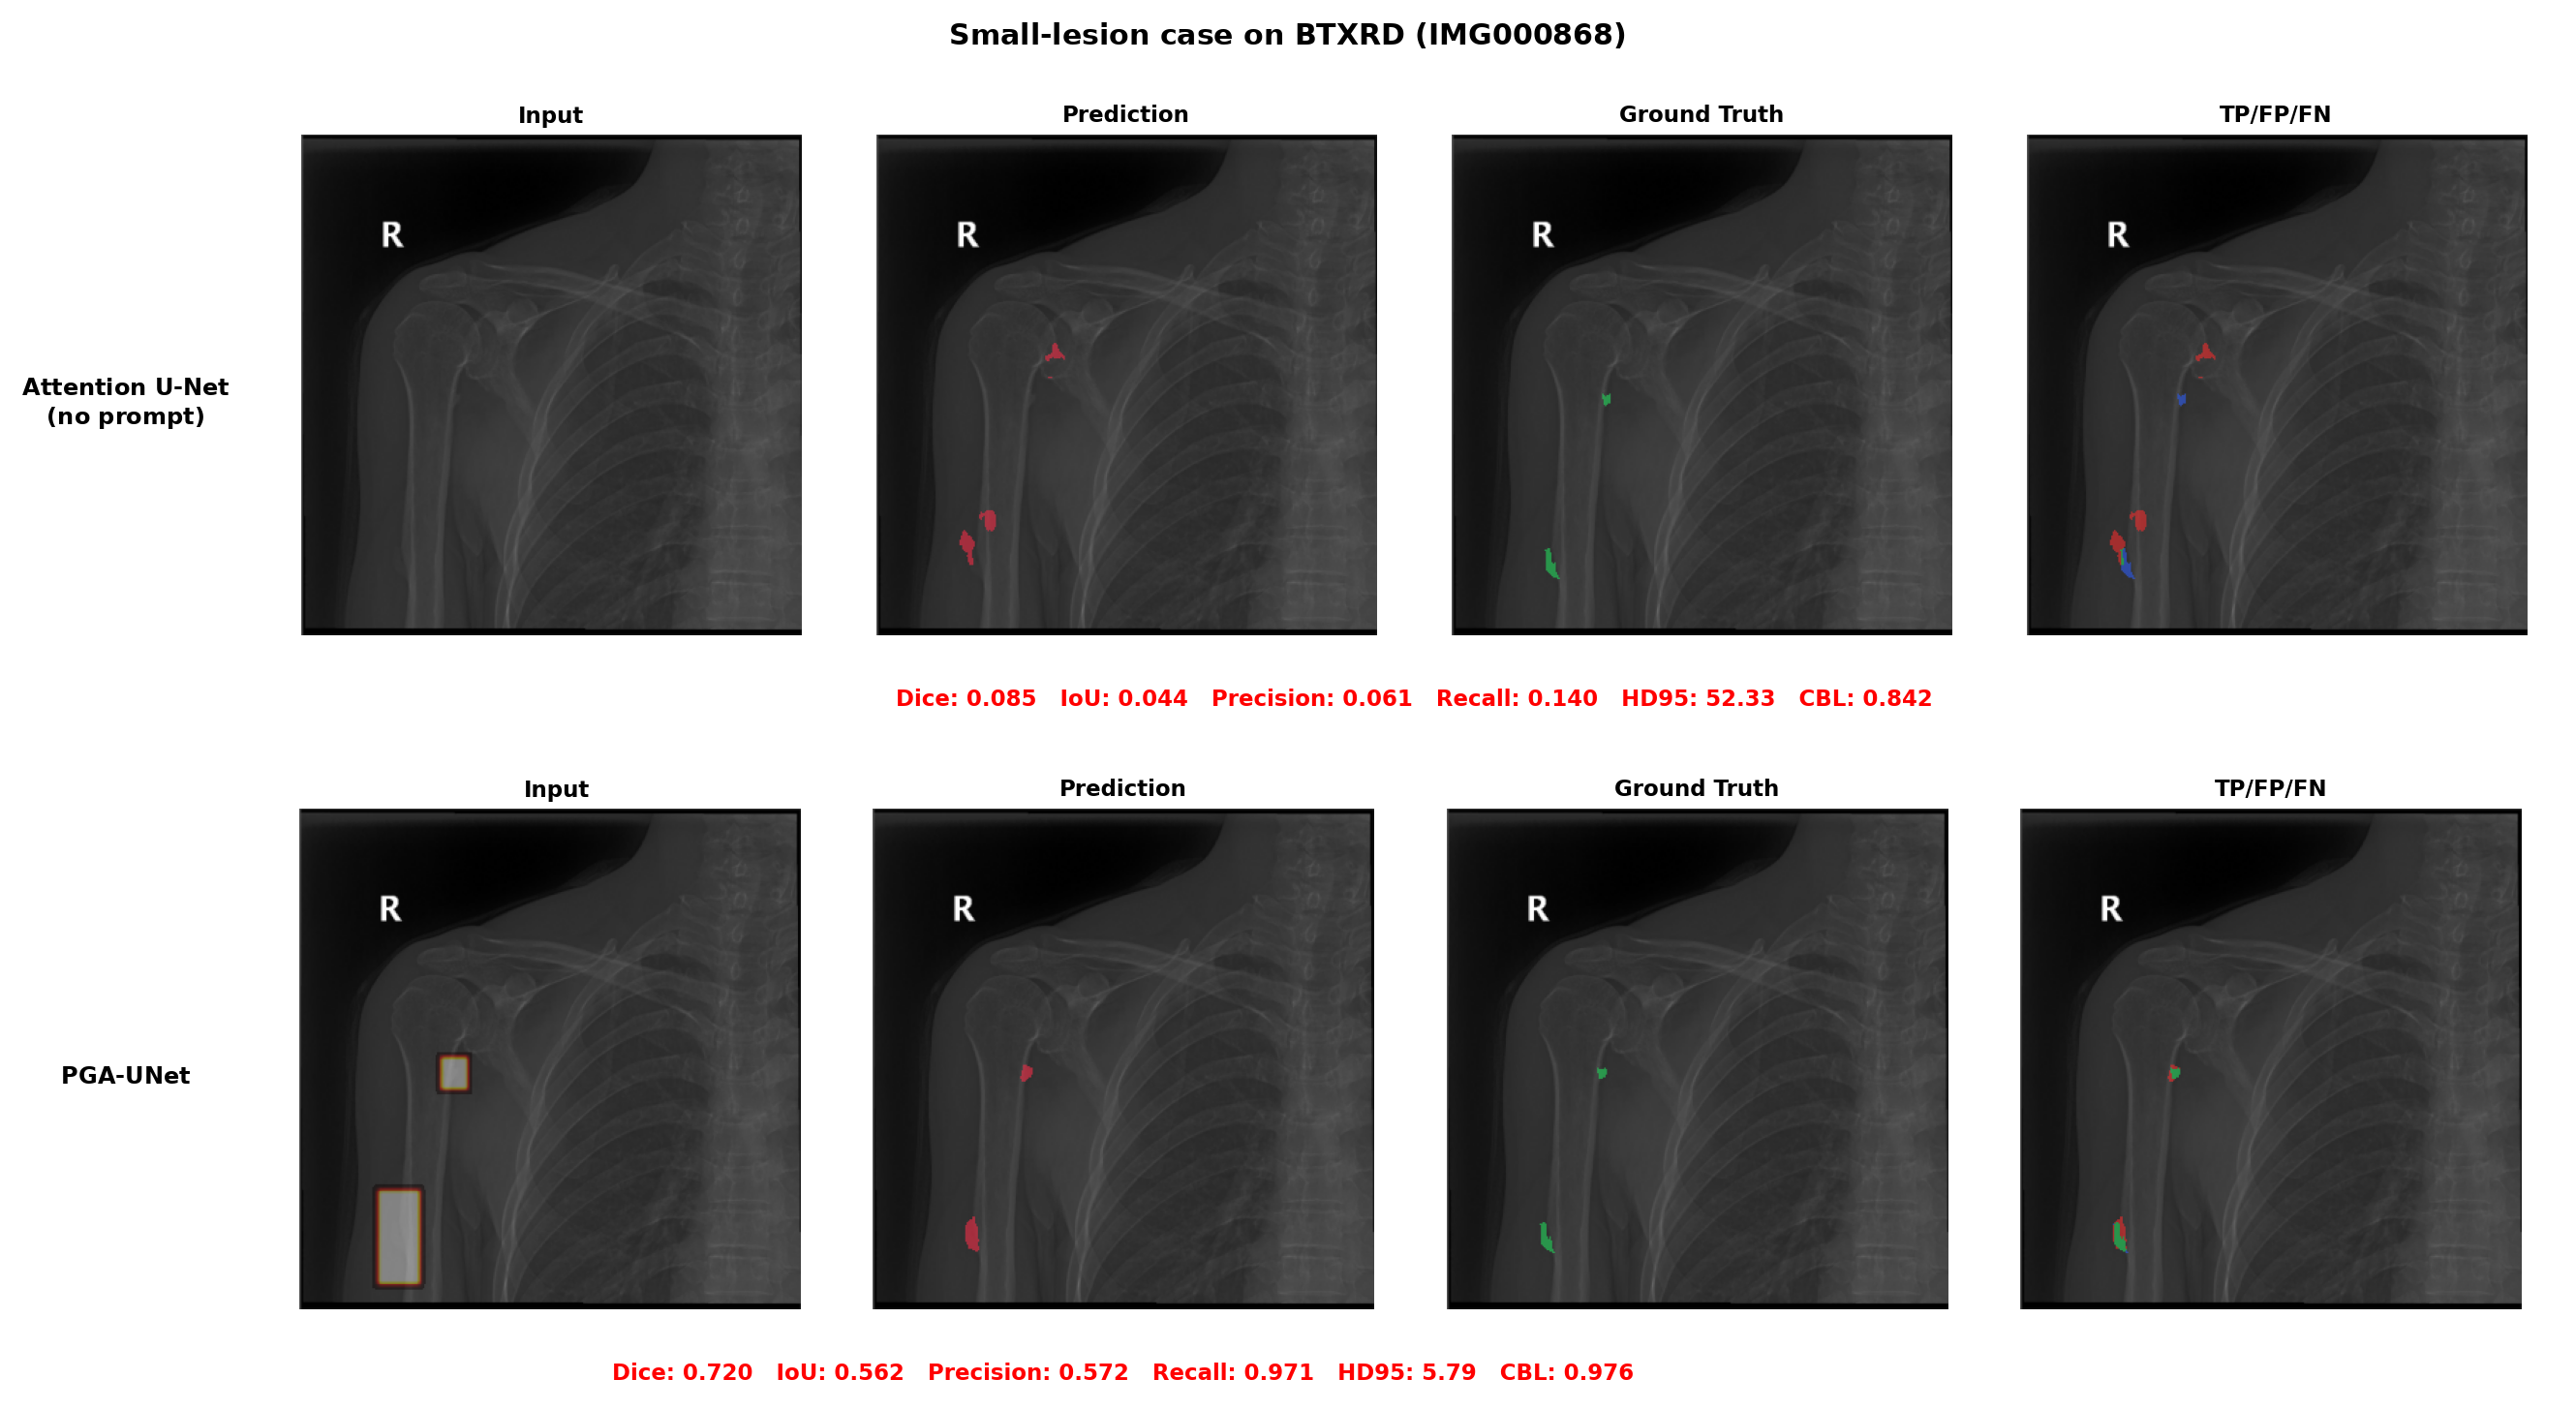
\includegraphics[width=\columnwidth]{images/results/small_lesion_pga_vs_attunet.png}
\caption{Small-lesion case on BTXRD (IMG000868, two GT polygons), Attention U-Net (no prompt) vs PGA-UNet, both at $512\times512$. Without a prompt, the automatic baseline all but misses both lesions (Dice 0.085); with a covering box prompt, PGA-UNet recovers them (Dice 0.720). The two conventional prompt baselines are quantified in Table~\ref{tab:small-att} but omitted here for readability.}
\label{fig:small-att}
\end{figure}

\paragraph{Resolution on the small-lesion images}
This same fixed set of 50 images per dataset is held constant and evaluated in turn at $128$, $256$, and $512$; predictions and ground truth are merged at image level at each resolution, HD95 is reported both in native pixels and in normalized form, and the degradation is measured relative to the $512$ result. On these images, PGA-UNet's Dice falls from 0.766 at $512$ to 0.631 at $128$ on BTXRD, and from 0.720 to 0.609 on FracAtlas; the loss from $512$ to $128$ is 0.135 and 0.111 respectively (Table~\ref{tab:small-res}). On BTXRD this loss is larger than the 0.068 lost over the same resolution range on the full test set (Table~\ref{tab:resolution}); on FracAtlas the full-test loss is itself large (0.131), so the loss on this subgroup is comparable rather than larger there. As with the full-resolution comparison above, each configuration is scored in its own frame, so this combines resolution and mask-sampling effects rather than isolating either.

\begin{table}[t]
\caption{PGA-UNet on the fixed 50-image lower-lesion-area image subset of each dataset across resolutions. Dice, IoU, and CBL are reported as covering / off-center; each configuration is scored in its own frame. The HD95 pair denotes native pixels / normalized distance under the covering condition. The Delta Dice column is the covering-prompt difference relative to the $512$ configuration.}
\label{tab:small-res}
\centering
\scriptsize
\resizebox{\columnwidth}{!}{%
\begin{tabular}{llccccc}
\toprule
Dataset & Res. & Dice & IoU & CBL & HD95$_\mathrm{px}$\,/\,$_n$ & $\Delta$Dice \\
\midrule
\multirow{3}{*}{BTXRD}
& $128$ & 0.631 / 0.662 & 0.488 / 0.517 & 0.738 / 0.758 & 3.9 / 0.022 & $-0.135$ \\
& $256$ & 0.714 / 0.695 & 0.570 / 0.548 & 0.869 / 0.849 & 7.2 / 0.020 & $-0.052$ \\
& $512$ & \textbf{0.766} / \textbf{0.757} & \textbf{0.637} / \textbf{0.627} & \textbf{0.897} / \textbf{0.890} & 14.0 / 0.019 & --- \\
\midrule
\multirow{3}{*}{FracAtlas}
& $128$ & 0.609 / 0.543 & 0.462 / 0.393 & 0.828 / 0.757 & 8.9 / 0.049 & $-0.111$ \\
& $256$ & 0.642 / 0.610 & 0.484 / 0.451 & 0.887 / 0.845 & 10.3 / 0.029 & $-0.079$ \\
& $512$ & \textbf{0.720} / \textbf{0.712} & \textbf{0.578} / \textbf{0.570} & \textbf{0.907} / \textbf{0.893} & 8.3 / 0.012 & --- \\
\bottomrule
\end{tabular}
}
\end{table}

\begin{figure}[t]
\centering
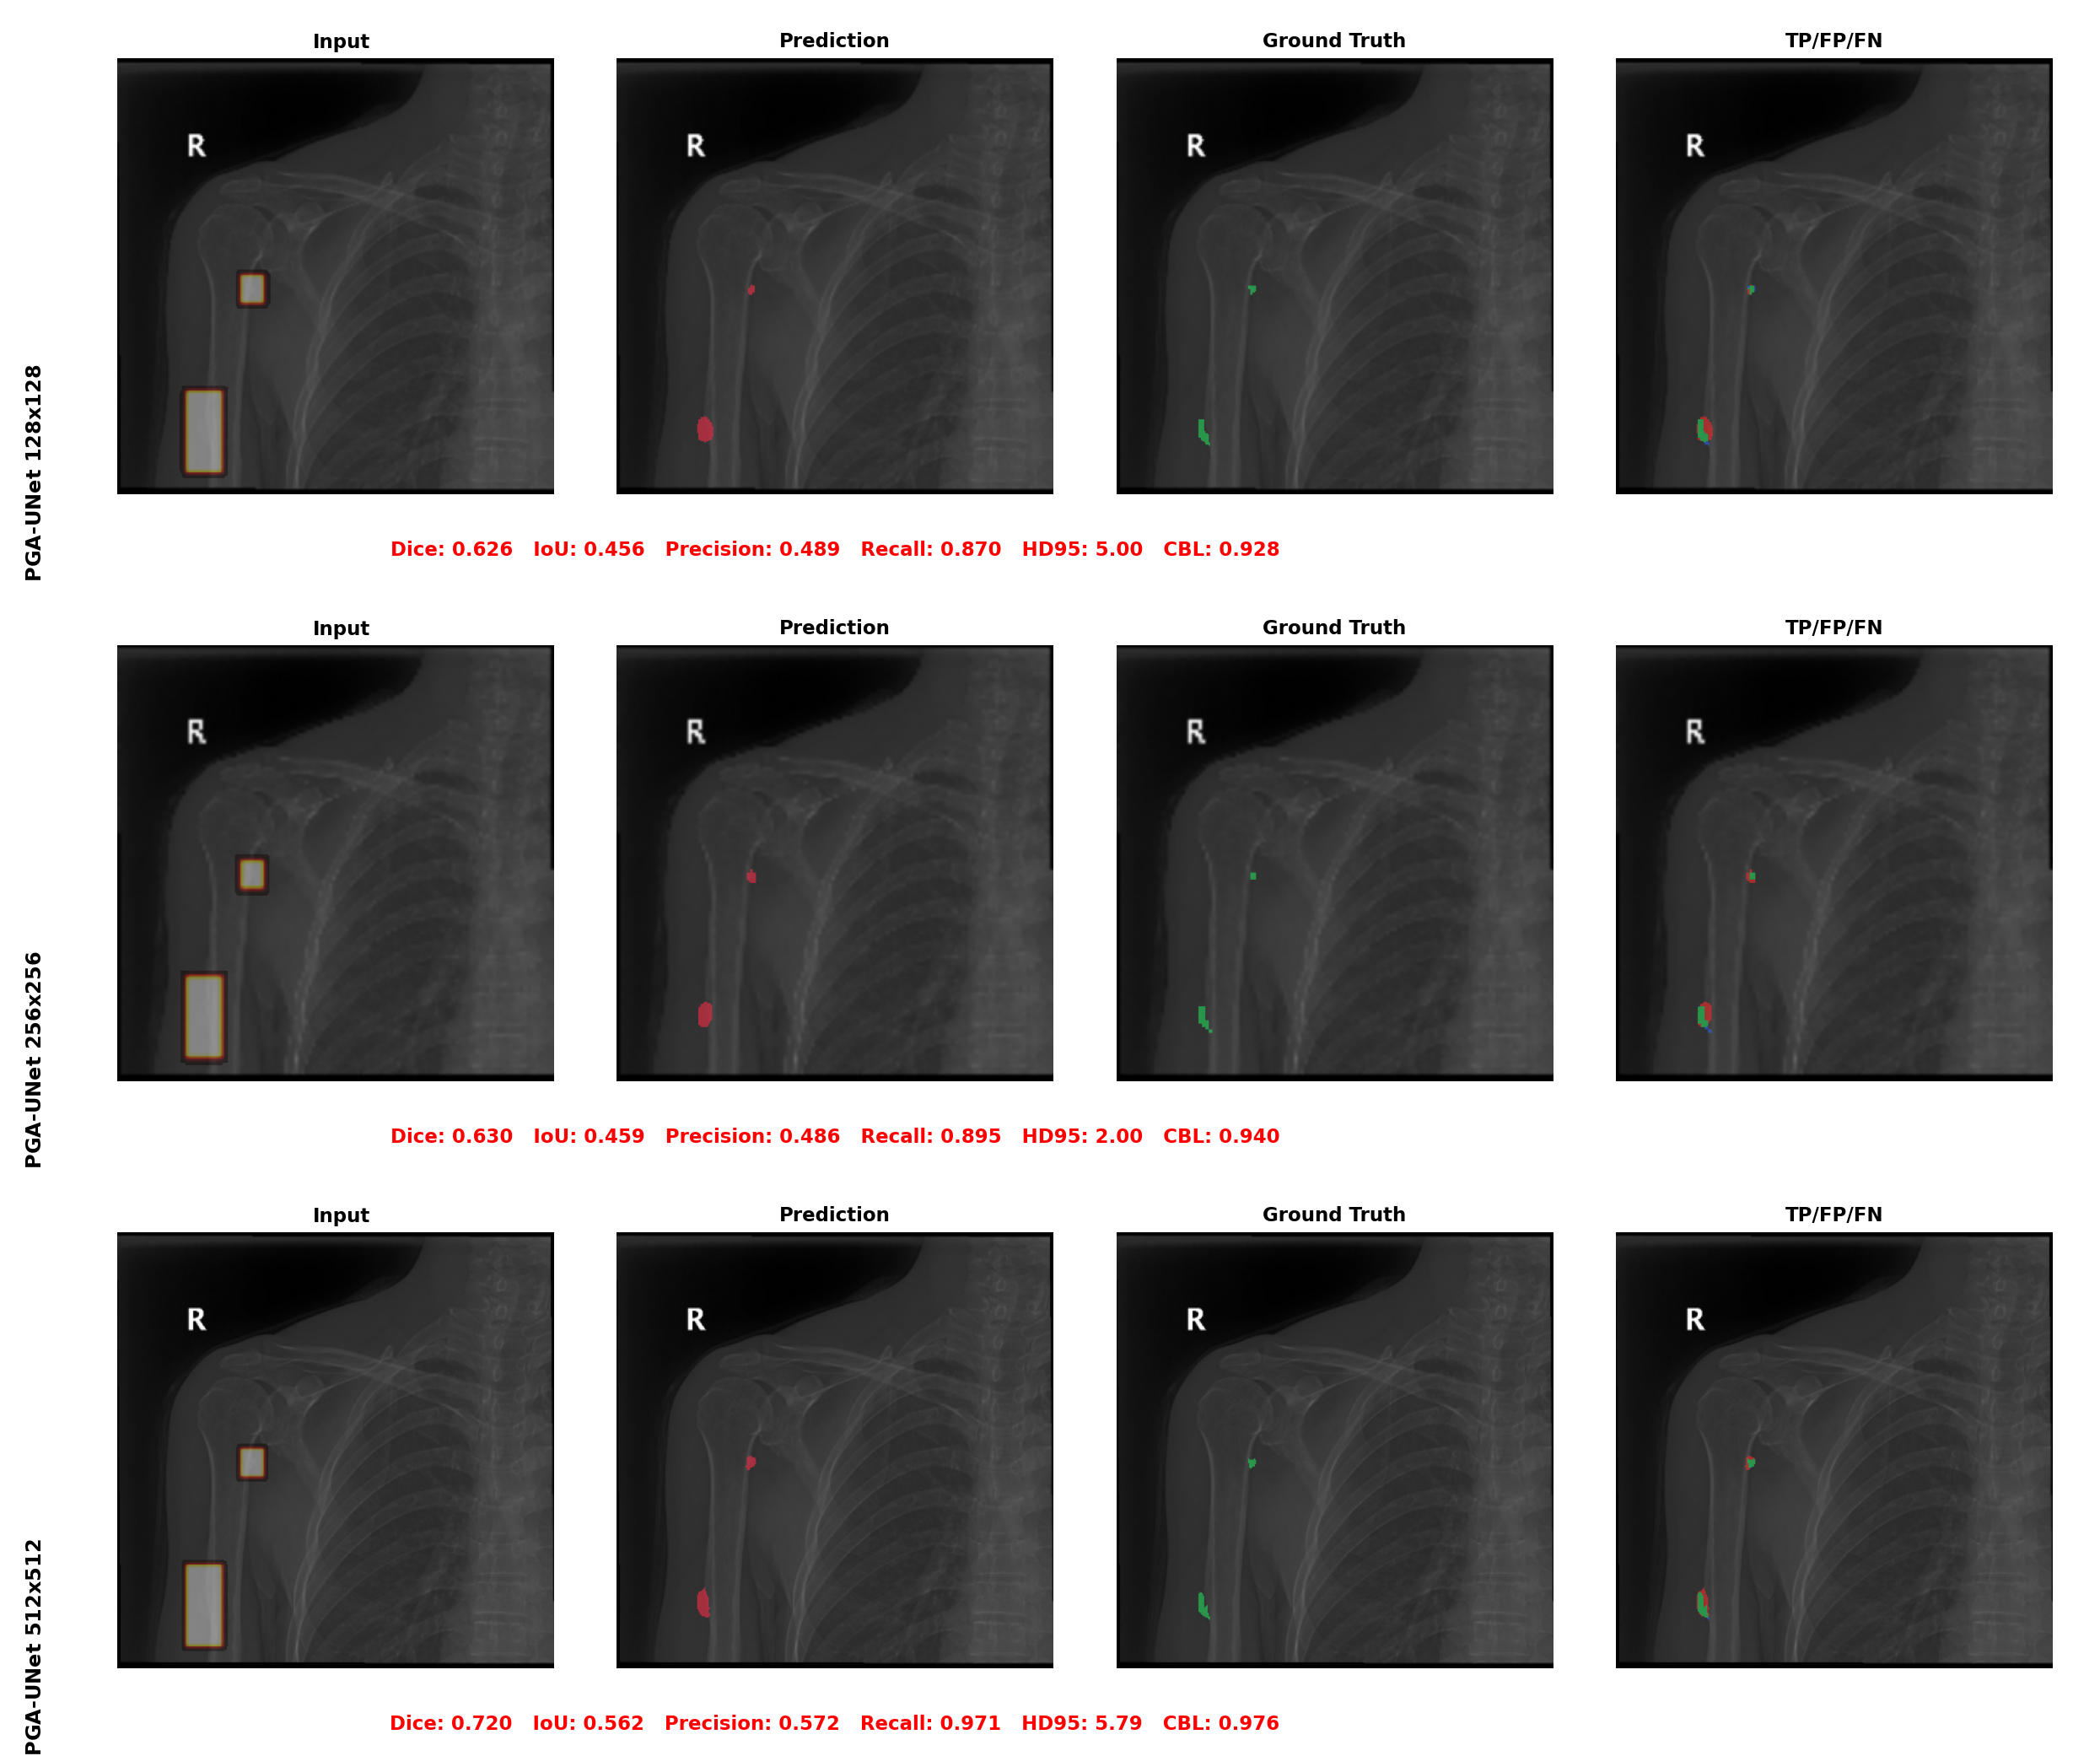
\includegraphics[width=\columnwidth]{images/results/small_lesion_pga_128_256_512.png}
\caption{PGA-UNet on the same small-lesion case on BTXRD (IMG000868, two GT polygons) at $128\times128$, $256\times256$, and $512\times512$ (Dice 0.626, 0.630, 0.720). The prediction tightens around the lesion as resolution increases.}
\label{fig:small-res}
\end{figure}

On this lower-lesion-area image subset, PGA-UNet's margin over the no-prompt baseline remains large on both datasets, and the resolution effect is larger than on the full test set on BTXRD; on FracAtlas the full test set already loses this much to resolution, so the subgroup does not show a further resolution penalty there. As noted above, this subset is a descriptive selection of images and does not by itself establish that the method preferentially benefits small lesions in general.

\subsection{Sensitivity to Prompt Displacement}
\label{sec:robust}
Under the predefined off-center construction, PGA-UNet's Dice decreases by 0.008 on BTXRD and 0.014 on FracAtlas (Table~\ref{tab:robust}); on the 50-image lower-lesion-area image subset of Section~\ref{sec:small} the decrease stays under 0.01 for both datasets. The binary channel baseline has a smaller decrease on FracAtlas (0.005), so the results do not establish that PGA-UNet is uniformly the least sensitive model to this construction; the crop baseline decreases more on FracAtlas (0.027) and about as much on BTXRD (0.008). PGA-UNet retains the highest observed Dice among the three configurations in this table under both prompt conditions on both datasets. These observations apply to the evaluated lesion-covering box construction and do not characterize arbitrary user-drawn, partial-coverage, or off-target prompts.

\begin{table*}[t]
\caption{Observed sensitivity to the predefined off-center box construction (z: covering, s: off-center). All configurations use a $512\times512$ input and scoring frame; crop predictions are mapped back to the full frame. The Delta Dice column is off-center minus covering Dice. Boxes preserve full lesion coverage, and the off-center construction may change box extent when needed to retain coverage. Results are descriptive point estimates on the fixed test splits.}
\label{tab:robust}
\centering
\begin{tabular}{llccccc}
\toprule
Dataset & Model & Dice z/s & $\Delta$Dice & IoU z/s & HD95 z/s & CBL z/s \\
\midrule
\multirow{3}{*}{BTXRD}
& U-Net + binary prompt channel & 0.760 / 0.748 & $-0.012$ & 0.635 / 0.626 & 33.0 / 32.6 & 0.895 / 0.890 \\
& Attention U-Net + prompt crop & 0.741 / 0.733 & $-0.008$ & 0.615 / 0.607 & 24.7 / 26.4 & 0.912 / 0.896 \\
& PGA-UNet & \textbf{0.782 / 0.774} & $-0.008$ & \textbf{0.661 / 0.652} & \textbf{22.8} / 24.5 & \textbf{0.918 / 0.912} \\
\midrule
\multirow{3}{*}{FracAtlas}
& U-Net + binary prompt channel & 0.593 / 0.588 & $\mathbf{-0.005}$ & 0.434 / 0.428 & 22.9 / 24.0 & 0.887 / 0.860 \\
& Attention U-Net + prompt crop & 0.590 / 0.563 & $-0.027$ & 0.451 / 0.428 & 22.0 / 23.8 & 0.865 / 0.833 \\
& PGA-UNet & \textbf{0.727 / 0.713} & $-0.014$ & \textbf{0.585 / 0.570} & \textbf{10.5} / \textbf{10.4} & \textbf{0.913 / 0.897} \\
\bottomrule
\end{tabular}
\end{table*}

For reference, the no-prompt Attention U-Net is by construction unaffected by this box displacement (0.517 on BTXRD, 0.342 on FracAtlas under both conditions), and the three fine-tuned promptable reference models, each scored in its own native frame, lose 0.03 to 0.08 Dice under the same off-center construction (SAM-Med2D: $-0.029$ BTXRD / $-0.031$ FracAtlas; MedSAM: $-0.033$ / $-0.063$; ScribblePrompt-UNet: $-0.080$ / $-0.081$); these three are not included in Table~\ref{tab:robust} because their scoring frames differ from the shared $512\times512$ frame used there.

\begin{figure}[t]
\centering

\includegraphics[width=\columnwidth]{images/results/prompt_robustness_examples.png}
\caption{PGA-UNet on the same BTXRD case (IMG000020) under a covering prompt (top) and an off-center prompt (bottom); Dice is unchanged at 0.942.}
\label{fig:robust}
\end{figure}

\subsection{Ablation Study}
\label{sec:ablation}
The ablation drops one factor at a time from the full model (Gaussian prompt combined with PSG and CAD), and separately tests replacing the Gaussian prompt with a binary box (Table~\ref{tab:ablation}). The full model is first or second in all four dataset-and-prompt combinations; each ablated variant is top-two in exactly one. The binary-box variant leads BTXRD covering by 0.006 Dice but trails by 0.059 on FracAtlas, and PSG-only is close to the full model on BTXRD yet falls 0.092 Dice below it on FracAtlas. These are single-split results.

\begin{table*}[t]
\caption{Ablation at $512\times512$, image-level merged, single split. Dice, IoU, HD95 and CBL as covering / off-center.}
\label{tab:ablation}
\centering
\begin{tabular}{llcccc}
\toprule
Dataset & Configuration & Dice & IoU & HD95 & CBL \\
\midrule
\multirow{5}{*}{BTXRD}
& CAD only & 0.771 / 0.759 & 0.649 / 0.635 & 23.1 / 24.2 & 0.915 / 0.905 \\
& PSG only & 0.779 / 0.771 & 0.660 / 0.651 & 29.4 / 28.4 & 0.908 / 0.902 \\
& PSG + vanilla attention gate & 0.769 / 0.757 & 0.645 / 0.633 & 26.4 / 28.7 & 0.906 / 0.896 \\
& Full model + binary box prompt & \textbf{0.788} / 0.770 & \textbf{0.668} / 0.651 & 23.1 / 28.5 & 0.914 / 0.900 \\
& Full PGA-UNet (Gaussian + PSG + CAD) & 0.782 / \textbf{0.774} & 0.661 / \textbf{0.652} & \textbf{22.8} / \textbf{24.5} & \textbf{0.918} / \textbf{0.912} \\
\midrule
\multirow{5}{*}{FracAtlas}
& CAD only & 0.696 / 0.685 & 0.551 / 0.540 & 18.0 / \textbf{12.0} & 0.903 / 0.885 \\
& PSG only & 0.635 / 0.611 & 0.479 / 0.459 & 14.5 / 14.8 & 0.894 / 0.857 \\
& PSG + vanilla attention gate & 0.690 / 0.691 & 0.548 / 0.547 & 14.0 / 14.1 & 0.892 / 0.881 \\
& Full model + binary box prompt & 0.668 / 0.657 & 0.514 / 0.505 & 12.0 / 13.2 & 0.904 / 0.886 \\
& Full PGA-UNet (Gaussian + PSG + CAD) & \textbf{0.727} / \textbf{0.713} & \textbf{0.585} / \textbf{0.570} & \textbf{10.5} / 10.4 & \textbf{0.913} / \textbf{0.897} \\
\bottomrule
\end{tabular}
\end{table*}

\begin{table}[t]
\caption{Paired comparison of the full model against each ablated variant, per-image Dice on the single split. The Delta column is the mean per-image Dice difference (full minus variant), tested with a two-sided paired sign-flip randomization test ($20{,}000$ permutations). $^{**}$ marks entries that stay significant ($p<0.05$) after Holm correction over the full family of ablation tests (four ablated model contrasts $\times$ two datasets $\times$ two prompt conditions, all on Dice, the only metric tested here); $^{*}$ marks raw $p<0.05$ that does not survive correction.}
\label{tab:ablation-sig}
\centering
\scriptsize
\resizebox{\columnwidth}{!}{%
\begin{tabular}{lcccc}
\toprule
$\Delta$Dice, full vs variant & \multicolumn{2}{c}{BTXRD} & \multicolumn{2}{c}{FracAtlas} \\
\cmidrule(lr){2-3}\cmidrule(lr){4-5}
 & covering & off-center & covering & off-center \\
\midrule
CAD only (no PSG)            & $+0.010$ & $+0.015^{*}$ & $+0.031^{*}$  & $+0.028^{*}$ \\
PSG only (no CAD)            & $+0.002$ & $+0.003$     & $+0.092^{**}$ & $+0.102^{**}$ \\
PSG + vanilla attention gate & $+0.012$ & $+0.017^{*}$ & $+0.038^{*}$  & $+0.022$ \\
Full + binary box prompt     & $-0.006$ & $+0.004$     & $+0.059^{**}$ & $+0.056^{**}$ \\
\bottomrule
\end{tabular}
}
\end{table}

The component effects depend on the dataset. On FracAtlas, the full configuration has higher Dice than the CAD-removed and binary-prompt variants, and these differences survive the reported Holm correction over the full family of ablation tests (Table~\ref{tab:ablation-sig}); the CAD-removed variant loses 0.09 to 0.10 Dice. On BTXRD, where every configuration already sits near 0.78, the reported Dice differences from the ablated variants do not survive that correction, including the 0.006 Dice binary-box lead (bootstrap $95\%$ CI $[-0.017, +0.004]$); the binary-prompt variant also has a higher covering-prompt point estimate than the Gaussian configuration there. The ablations therefore support dataset-dependent benefits of the complete conditioning design, without establishing that every component is necessary in every setting. They do not directly measure preservation of weak lesion features or estimate variation across training seeds, and a single split could not settle finer, component-by-component contributions in any case.

\begin{figure}[t]
\centering

\includegraphics[width=\columnwidth]{images/ablation/ablation_gaussian_vs_binary_case.png}
\caption{Full PGA-UNet on the same BTXRD case (IMG000054) with a Gaussian-plateau prompt vs a binary box prompt, both at $512\times512$. The binary variant loses localization even though PSG and CAD are unchanged.}
\label{fig:ablation-gaussian-binary}
\end{figure}

\subsection{Monte Carlo Cross-Validation}
\label{sec:mccv}
We retrained PGA-UNet at $512\times512$ on four additional random image-level splits, keeping the training seed fixed at 22120196 and changing only the split seed (Table~\ref{tab:mccv}). Across these splits, PGA-UNet obtains covering-prompt Dice of $0.769\pm0.005$ on BTXRD and $0.733\pm0.007$ on FracAtlas, and off-center Dice of $0.762\pm0.004$ and $0.728\pm0.011$, respectively (mean $\pm$ standard deviation); CBL varies with a standard deviation of at most 0.013. These results characterize PGA-UNet's own observed split-to-split variation; they do not establish comparable variation for the baselines, which were not retrained across these splits, or the stability of the differences from competing models reported elsewhere in this article.

\begin{table}[t]
\caption{Monte Carlo cross-validation of PGA-UNet at $512\times512$, four repeated random image-level splits, mean $\pm$ standard deviation.}
\label{tab:mccv}
\centering
\scriptsize
\resizebox{\columnwidth}{!}{%
\begin{tabular}{llcccc}
\toprule
Dataset & Prompt & Dice & IoU & HD95 & CBL \\
\midrule
\multirow{2}{*}{BTXRD}
& Covering & $0.769\pm0.005$ & $0.647\pm0.006$ & $25.0\pm2.5$ & $0.905\pm0.005$ \\
& Off-center & $0.762\pm0.004$ & $0.639\pm0.007$ & $25.7\pm2.0$ & $0.901\pm0.007$ \\
\midrule
\multirow{2}{*}{FracAtlas}
& Covering & $0.733\pm0.007$ & $0.595\pm0.007$ & $14.1\pm2.7$ & $0.909\pm0.006$ \\
& Off-center & $0.728\pm0.011$ & $0.590\pm0.010$ & $15.6\pm3.9$ & $0.904\pm0.013$ \\
\bottomrule
\end{tabular}
}
\end{table}

\subsection{Training-Seed Stability Analysis}
\label{sec:seedstability}
The Monte Carlo cross-validation above varies the image-level split while keeping the training seed fixed at 22120196. To characterize the complementary source of variability, training-run randomness itself, we are separately retraining PGA-UNet at $512\times512$ on the original fixed split (Table~\ref{tab:splits}) using three additional training seeds, with every other setting from Section~\ref{sec:training} held fixed. All four runs use the same fixed train/validation/test partition; only the seed governing weight initialization, data shuffling, and other stochastic training behavior changes between them.

This analysis is restricted to PGA-UNet. None of the evaluated baselines, the two conventional prompt baselines or the three promptable foundation models, has been retrained across multiple seeds, so no comparison in this article claims stable superiority over those baselines across training seeds. Of the three additional seeds, one (19122003) has completed on both datasets at the time of this draft; the other two are still training. Table~\ref{tab:seedstability} therefore reports an interim mean $\pm$ sample standard deviation over the $n=2$ completed seeds (22120196 and 19122003), not the full four; the sample size is stated in the caption, and the table will be extended with the remaining two seeds, not recomputed from scratch, once they complete (see \texttt{PENDING\_MULTISEED.md}).

\begin{table*}[t]
\caption{Training-seed stability of PGA-UNet at $512\times512$ on the original fixed split (Table~\ref{tab:splits}). Interim results from $n=2$ completed training seeds (22120196 and 19122003) of the four planned; mean $\pm$ sample standard deviation ($\mathrm{ddof}=1$). Two additional seeds are still training and are not included here. Precision and recall are the standard pixel-level values for the image-level merged mask, reported only in this table; they are not a lesion-level detection recall, which this article does not measure. See \texttt{PENDING\_MULTISEED.md}.}
\label{tab:seedstability}
\centering
\scriptsize
\begin{tabular}{llcccccc}
\toprule
Dataset & Prompt & Dice & IoU & Precision & Recall & HD95 & CBL \\
\midrule
\multirow{2}{*}{BTXRD}
& Covering (\texttt{center\_zoom}) & $0.771\pm0.016$ & $0.645\pm0.022$ & $0.745\pm0.024$ & $0.831\pm0.000$ & $23.6\pm1.2$ & $0.914\pm0.005$ \\
& Off-center (\texttt{center\_shift}) & $0.762\pm0.017$ & $0.637\pm0.021$ & $0.747\pm0.024$ & $0.819\pm0.002$ & $24.8\pm0.5$ & $0.907\pm0.007$ \\
\midrule
\multirow{2}{*}{FracAtlas}
& Covering (\texttt{center\_zoom}) & $0.728\pm0.001$ & $0.586\pm0.002$ & $0.678\pm0.008$ & $0.835\pm0.011$ & $10.6\pm0.1$ & $0.908\pm0.006$ \\
& Off-center (\texttt{center\_shift}) & $0.713\pm0.001$ & $0.570\pm0.000$ & $0.674\pm0.007$ & $0.806\pm0.004$ & $11.0\pm0.8$ & $0.899\pm0.002$ \\
\bottomrule
\end{tabular}
\end{table*}

With only two completed seeds, these standard deviations are not yet informative about the true seed-to-seed spread and should not be read as a stable estimate; they describe only the two runs observed so far. Read as a two-point comparison, not a distribution: the newly completed seed's Dice is about 0.02 lower than the original seed's on BTXRD under both prompt conditions, while on FracAtlas the two seeds are within 0.002 Dice of each other. Between the two completed seeds, Precision differs by about 0.034 on BTXRD under both prompt conditions and by 0.010 to 0.012 on FracAtlas, while Recall differs by 0.001 to 0.002 on BTXRD and by 0.006 to 0.016 on FracAtlas. HD95 differs by about 1 to 2 pixels on BTXRD covering and by about 1 pixel on FracAtlas off-center, and by under 1 pixel on the other two rows. The picture is not uniform across metrics: Dice and Precision differ more between the two seeds on BTXRD than on FracAtlas, while Recall differs less on BTXRD than on FracAtlas. Whether any of these patterns hold up is exactly what the two remaining seeds will show; nothing here yet supports a general claim about which dataset or metric is more sensitive to the training seed.

\subsection{Efficiency}
\label{sec:efficiency}
PGA-UNet contains approximately 2.96 million parameters (Table~\ref{tab:efficiency}), about 92 times fewer than fine-tuned SAM-Med2D's 271.24 million. In the reported Tesla T4, batch-size-one measurement, a single forward pass takes 8.7 ms at $256\times256$ and 18.5 ms at $512\times512$; the evaluated SAM-Med2D configuration takes 50.3 ms at $256\times256$. ScribblePrompt-UNet takes 6.2 ms at its $128\times128$ input, with 3.99 million parameters, a closer parameter count to PGA-UNet's than SAM-Med2D's; MedSAM's $1024\times1024$ input gives it the highest GFLOPs and latency in the group even though it has far fewer parameters than SAM-Med2D. Quality at these same per-model resolutions is reported separately in Tables~\ref{tab:sam} and \ref{tab:sam-ref}; a smaller parameter count or lower latency here does not by itself imply better segmentation, and those tables should be read together, not this one alone, when weighing a model choice. Latency is measured in FP32 with synthetic random-tensor inputs at each model's own resolution, not real images; each GPU figure is the mean over 50 timed forward passes after 10 warmup passes, with \texttt{torch.cuda.synchronize()} called after warmup and after every timed pass, and each CPU figure is the mean over 20 timed passes after 5 warmup passes on the same machine. The specific CPU model was not captured by the benchmark script and is not available to report. These measurements describe the tested implementations on one specific GPU and do not rank complete interactive workflows. They do not include a separate analysis of first-prompt versus cached subsequent-prompt operation, which would matter for the SAM-family models since they can reuse one image embedding across several prompts on the same image, and a single forward-pass time is not the latency of the perturbation-based self-assessment score or candidate shortlist, which each require several forward passes.

\begin{table}[t]
\caption{Parameters, FLOPs, and single forward-pass latency in the tested environment (NVIDIA Tesla T4, batch size 1), one BTXRD checkpoint per model.}
\label{tab:efficiency}
\centering
\scriptsize
\resizebox{\columnwidth}{!}{%
\begin{tabular}{lcccc}
\toprule
Model & Params & GFLOPs & GPU ms & CPU ms \\
\midrule
PGA-UNet $256$ & 2.96M & 7.74 & 8.7 & 93.6 \\
PGA-UNet $512$ & 2.96M & 30.97 & 18.5 & 341.7 \\
SAM-Med2D $256$ & 271.24M & 92.02 & 50.3 & 1343.6 \\
MedSAM $1024$ & 93.74M & 976.48 & 381.7 & 12129.4 \\
ScribblePrompt $128$ & 3.99M & 32.81 & 6.2 & 187.4 \\
\bottomrule
\end{tabular}
}
\end{table}

\subsection{Exploratory Comparison of Segmentation Losses}
\label{sec:loss}
Because the segmentation targets in this article are small, we tried replacing the Dice term with a size-conditioned Tversky loss, and in another trial, with a Focal Dice loss, with every other setting held fixed (Table~\ref{tab:loss}). Neither option worked better on Dice, which is best or tied for the default Dice + BCE objective on both datasets and both prompt conditions; HD95 follows the same pattern. CBL mostly favors the default too, with one exception: on FracAtlas covering, Tversky's CBL (0.918) is slightly higher than the default's (0.913), even though its Dice, IoU, and HD95 are all worse there. Focal Dice is a clear step backward on FracAtlas on every metric, with HD95 exceeding 100 pixels. We treat this as a negative control: under the current protocol, the default objective remains the better choice on the metric it is trained to optimize, and neither alternative is adopted.

\begin{table}[t]
\caption{Exploratory segmentation-loss comparison for PGA-UNet at $512\times512$, everything else fixed. Dice, IoU, HD95, and CBL as covering / off-center. The default is not changed.}
\label{tab:loss}
\centering
\scriptsize
\resizebox{\columnwidth}{!}{%
\begin{tabular}{llcccc}
\toprule
Dataset & Loss & Dice & IoU & HD95 & CBL \\
\midrule
\multirow{3}{*}{BTXRD}
& Dice + BCE (default) & \textbf{0.782} / \textbf{0.774} & \textbf{0.661} / \textbf{0.652} & 22.8 / 24.5 & \textbf{0.918} / \textbf{0.912} \\
& Size-conditioned Tversky & 0.778 / 0.767 & 0.660 / 0.649 & 25.2 / 30.3 & 0.916 / 0.903 \\
& Focal Dice & 0.773 / 0.765 & 0.649 / 0.642 & 25.6 / 25.6 & 0.913 / 0.907 \\
\midrule
\multirow{3}{*}{FracAtlas}
& Dice + BCE (default) & \textbf{0.727} / \textbf{0.713} & \textbf{0.585} / \textbf{0.570} & \textbf{10.5} / \textbf{10.4} & 0.913 / \textbf{0.897} \\
& Size-conditioned Tversky & 0.709 / 0.680 & 0.561 / 0.530 & 11.0 / 12.2 & \textbf{0.918} / 0.888 \\
& Focal Dice & 0.642 / 0.578 & 0.493 / 0.425 & 105.5 / 110.1 & 0.802 / 0.732 \\
\bottomrule
\end{tabular}
}
\end{table}

\subsection{Failure Modes}
\label{sec:failure}
PGA-UNet still makes mistakes, and these mistakes are not random but recur in a few patterns. In qualitative review, low Dice tends to cluster on lesions that are elongated or branching, lesions located in cluttered anatomy such as the shoulder or clavicle, or lesions that barely stand out from the surrounding bone. In such cases, even a good covering box does not help if the local image evidence itself is too weak.

\begin{figure}[t]
\centering

\includegraphics[width=\columnwidth]{images/failure/failure_case_overlap.png}
\caption{Failure case on BTXRD (IMG000013, Dice 0.120): the prompt covers the lesion at the chest/rib margin, but PGA-UNet's prediction lands away from it. A covering box does not fix a case where the local image evidence is itself ambiguous.}
\label{fig:failure}
\end{figure}

\subsection{Training-Free Self-Assessment and Candidate Suggestion}
\label{sec:selfassess-results}
The two support signals below are computed directly from the trained model's output and are reported as preliminary. $Q$ (Section~\ref{sec:selfassess}) is computed without ground-truth masks at inference; on the annotated lesion-bearing test images, its association with per-prompt Dice is quantified by the correlations below (Table~\ref{tab:selfassess}). Each lesion polygon (one prompt) is treated as an independent unit in this correlation, permutation, and bootstrap analysis, at the sample sizes in Table~\ref{tab:splits} (e.g. 232 BTXRD test polygons); images with more than one lesion contribute one unit per polygon rather than one unit per image, and we have not adjusted the analysis for this within-image dependence. The Spearman correlation between $Q$ and the true Dice reaches 0.70 (covering) and 0.60 (off-center) on BTXRD, and 0.65 and 0.48 on FracAtlas; all four are significantly different from zero (permutation test, $p<0.001$), with bootstrap $95\%$ intervals ranging from $[0.61,0.77]$ on BTXRD covering to $[0.29,0.63]$ on FracAtlas off-center. Pearson correlation follows the same pattern (0.82 and 0.76 on BTXRD, 0.59 and 0.44 on FracAtlas); we report Spearman as the primary statistic since it does not assume a linear $Q$-Dice relationship. Both component cues contribute meaningfully: mask decisiveness alone already reaches a Spearman of nearly 0.4, jitter stability reaches about 0.5 to 0.6, and averaging the two cues is always at least as good as either alone. As a control, we also tried training a small head to directly regress the Dice; in this specific experiment it collapsed to a near-constant output, with Spearman under 0.2 on both datasets, so we did not adopt it here. This single comparison does not establish that a learned confidence head cannot work in general, only that this particular configuration did not.

\begin{table}[t]
\caption{Spearman correlation between each training-free cue and the true per-prompt Dice. $Q = \mathrm{mean}(S_\mathrm{sharp}, S_\mathrm{stab})$.}
\label{tab:selfassess}
\centering
\scriptsize
\resizebox{\columnwidth}{!}{%
\begin{tabular}{lcccc}
\toprule
 & \multicolumn{2}{c}{BTXRD} & \multicolumn{2}{c}{FracAtlas} \\
\cmidrule(lr){2-3}\cmidrule(lr){4-5}
Cue & cover & off-center & cover & off-center \\
\midrule
$S_\mathrm{sharp}$ (mask decisiveness) & 0.42 & 0.39 & 0.47 & 0.43 \\
$S_\mathrm{stab}$ (jitter stability) & 0.64 & 0.56 & 0.63 & 0.45 \\
$Q$ & \textbf{0.70} & \textbf{0.60} & \textbf{0.65} & \textbf{0.48} \\
\bottomrule
\end{tabular}
}
\end{table}

Used in the reverse direction, $Q$ can also rank 50 randomly sampled candidate boxes and keep only the best few (Table~\ref{tab:suggest}, Figure~\ref{fig:demo-suggest}). The best of the top five boxes covers 0.84 and 0.90 of the lesion area on average on BTXRD and FracAtlas, and reaches near-complete coverage ($\ge0.999$) for 67\% and 82\% of images respectively. To check that this ranking earns its keep, we compare against two baselines computed on the same sampled 50-box pool per image: a random-5 selection (mean of 2,000 resamples per image) and an oracle-5 that picks the 5 truly best-covering boxes, an upper bound no ranking rule could see without the ground truth. $Q$-ranking roughly doubles mean coverage over random selection (0.52 vs 0.23 on BTXRD, 0.62 vs 0.26 on FracAtlas) and raises the near-complete-coverage rate by 26 to 27 points (67\% vs 40\% on BTXRD, 82\% vs 55\% on FracAtlas), closing much of the gap to the oracle's 86\% and 89\%. This is only a scaffold for a small suggestion feature: $Q$ is not a true probability, the shortlist does not replace the clinician's own review, and as the next paragraph shows, it is only meaningful when a lesion is actually present.

\begin{table}[t]
\caption{Candidate-region shortlist: $Q$-ranking vs a random-5 baseline and an oracle-5 upper bound, all drawn from the same 50 prompt-free boxes sampled per image. Coverage is the fraction of lesion pixels inside a box; near-complete-cov.\ counts images whose best-of-5 box reaches $\ge0.999$ coverage (random-5 uses the mean over 2,000 resamples per image).}
\label{tab:suggest}
\centering
\scriptsize
\resizebox{\columnwidth}{!}{%
\begin{tabular}{llccc}
\toprule
Dataset & Method & Mean cov. & Best-of-5 cov. & Near-complete-cov. \\
\midrule
\multirow{3}{*}{BTXRD}
& $Q$-ranked & \textbf{0.52} & 0.84 & 66.8\% \\
& Random-5   & 0.23 & 0.67 & 40.4\% \\
& Oracle-5   & ---  & \textbf{0.98} & \textbf{86.1\%} \\
\midrule
\multirow{3}{*}{FracAtlas}
& $Q$-ranked & \textbf{0.62} & 0.90 & 81.9\% \\
& Random-5   & 0.26 & 0.74 & 55.0\% \\
& Oracle-5   & ---  & \textbf{0.97} & \textbf{88.9\%} \\
\bottomrule
\end{tabular}
}
\end{table}

$Q$ presupposes that a lesion lies inside the box. To probe this assumption, we ran the same 50-box sampling on the lesion-free images of each dataset (1879 tumor-free BTXRD images, 3366 fracture-free FracAtlas images), where no coverage is defined (Table~\ref{tab:boxquality-normal}). $Q$ does not stay reliably low: the median collapses toward zero, but about 28\% of boxes on BTXRD and 42\% on FracAtlas still exceed $Q = 0.5$. The per-image maximum $Q$ averages 0.85 on BTXRD and 0.90 on FracAtlas. Together with the reported proportions of high-scoring boxes, these results show that high $Q$ values can occur on lesion-free anatomy. $Q$ should therefore not be interpreted as evidence of lesion presence: it ranks how good a mask is once a lesion has been located, and does not by itself flag lesion absence. This pattern is consistent with the model's weights being learned only on lesion-bearing images, with no negative class. Adding lesion-free images to training is a direction we plan to develop.

\begin{table}[t]
\caption{Distribution of the self-assessment score $Q$ on lesion-free images, with 50 random boxes sampled per image. With no lesion present, coverage is undefined; only the distribution of $Q$ is reported.}
\label{tab:boxquality-normal}
\centering
\scriptsize
\resizebox{\columnwidth}{!}{%
\begin{tabular}{lccccc}
\toprule
Dataset & Lesion-free img. & Median $Q$ & p90 $Q$ & Boxes $Q\!\ge\!0.5$ & $\overline{Q_{\max}/\text{img}}$ \\
\midrule
BTXRD & 1879 & 0.00 & 0.75 & 28\% & 0.85 \\
FracAtlas & 3366 & 0.07 & 0.82 & 42\% & 0.90 \\
\bottomrule
\end{tabular}
}
\end{table}

\paragraph{Exploratory post-hoc gate: MedSigLIP}
As one exploratory response to the finding above, we tested whether a separate, off-the-shelf vision-language model could catch some of the false-positive boxes that $Q$ misses on lesion-free images. This check uses BTXRD only, not FracAtlas, and reuses the same trained PGA-UNet $512\times512$ checkpoint as the rest of this article. We scored 50 sampled boxes per image with MedSigLIP \cite{b18}, a medical image-text encoder, used zero-shot as a post-hoc gate applied after PGA-UNet's prediction, not as part of the architecture and not fine-tuned. A fixed ensemble of positive and negative text prompts yields a cosine-margin score, thresholded at a cutoff chosen only on a validation split of 410 lesion-free images to retain 95\% of positive validation boxes; the held-out test images play no part in choosing this threshold. The held-out test split is the remaining 1{,}469 of the same 1{,}879 lesion-free BTXRD images used above, giving 73{,}450 sampled boxes.

Gating with MedSigLIP lowers the box-level false-positive rate on these held-out boxes from 61.96\% to 44.62\%, an absolute reduction of 17.33 points (paired cluster-bootstrap $95\%$ CI $[16.68, 17.98]$; Table~\ref{tab:medsiglip-gate}). On the article's own BTXRD test-split lesion boxes (232 boxes from 187 images, built with the same covering-box construction used throughout this article), the gate retains 96.12\% of positive boxes (cluster-bootstrap $95\%$ CI $[93.42, 98.30]$). Image-level false-positive rate, the fraction of lesion-free images with at least one surviving false-positive box among the 50 sampled, barely moves, from 100\% to 99.93\%: nearly every lesion-free image still has at least one box that fools the gated system. We do not report a post-gate Dice or other segmentation-quality measure here. This result is exploratory and supplementary, not a core contribution of this article: a lightweight external gate can reduce box-level false responses while keeping most positive boxes, without solving image-level false-positive detection; developing a purpose-built, better-calibrated lightweight gate is future work (Section~\ref{sec:discussion}).

\begin{table}[t]
\caption{MedSigLIP zero-shot post-hoc gate on BTXRD lesion-free images (held-out test split, 1{,}469 images, 50 boxes/image, 73{,}450 boxes). Positive-box retention is measured separately on the article's own BTXRD test-split lesion boxes (232 boxes, 187 images). Exploratory, not a core contribution; no post-gate Dice is reported.}
\label{tab:medsiglip-gate}
\centering
\scriptsize
\resizebox{\columnwidth}{!}{%
\begin{tabular}{lcc}
\toprule
Quantity & Before gate & After gate \\
\midrule
Box FPR (73{,}450 boxes) & 61.96\% & 44.62\% \\
Image FPR (1{,}469 images) & 100\% & 99.93\% \\
Positive-box retention (232 boxes) & \multicolumn{2}{c}{96.12\%} \\
\bottomrule
\end{tabular}
}
\end{table}

\begin{figure*}[t]
\centering
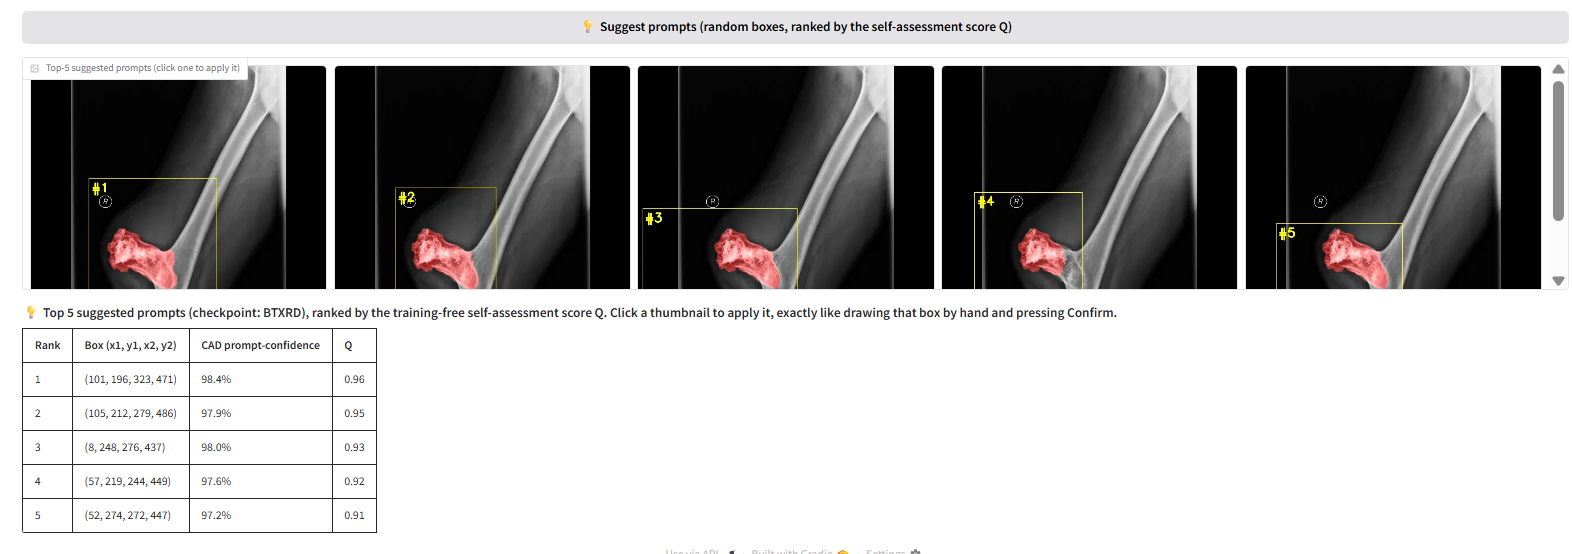
\includegraphics[width=\textwidth]{images/demo/demo_suggestion_btxrd.png}
\caption{Candidate-region shortlist on a BTXRD case. Fifty boxes are sampled with no prompt, scored by the self-assessment score $Q$, and the five highest-scoring boxes are shown for the clinician to accept, adjust, or reject. A FracAtlas case is shown in the supplementary material.}
\label{fig:demo-suggest}
\end{figure*}


\section{Discussion}
\label{sec:discussion}
The question this article set out to answer was never simply whether a prompt is useful in general. The real question is: once a coarse box has already narrowed the search, does the way the model handles that prompt still matter? Attention U-Net without a box answers a different question altogether, and its low Dice, near 0.34 on FracAtlas, measures only how much of the task is finding the lesion. The design is tested wherever the same box is given to another model or stripped of a component: the prompt-matched Attention U-Net baselines, the fine-tuned promptable foundation models, and the ablation. Across all of them, PGA-UNet keeps a margin that is modest on BTXRD, clearer on FracAtlas, and largest on the Attention U-Net bottom-Dice group and on the smallest lesions. If the point of keeping the prompt active through the encoder and decoder is to preserve a faint lesion signal, it should help most where that signal is faintest, and that is the direction the results take: the margin over prompt-matched baselines, the per-component ablation gaps, and the robustness to prompt displacement are all largest on FracAtlas, on the smallest lesions, and under off-center prompts, and all shrink toward the easy end. The consistency of that direction across independent measurements is the main support for the design, more than any single comparison.

Beyond the main result, the study also yields two side findings. First, the loss comparison gives a fairly clear negative result: neither the size-conditioned Tversky loss nor the Focal Dice loss helps, and Focal Dice even makes things distinctly worse on FracAtlas, so we keep the default Dice + BCE objective. Second, the self-assessment score gives a moderate positive result: $Q$ correlates with the true Dice at a rank level of about 0.5 to 0.7 without needing any label at all, and it succeeds where a small learned regression head does not, since that head ultimately just predicts a mean value. Even so, $Q$ remains only a heuristic number, not yet calibrated, so the candidate list built from it should only be used to suggest where a clinician might look first, not to replace self-detection.

This study also has fairly concrete limitations. Inputs are resized to a fixed square, and the resolution results themselves show that this genuinely costs accuracy on the smallest lesions. The prompts in this article are all drawn from existing annotations, not directly drawn by a radiologist, and the protocol assumes the user has already found the correct region before drawing a box over it. Cases where the box only partially covers the lesion, is negative, or targets the wrong region are not addressed by this article; a direct check shows that the self-assessment score $Q$ in particular stays high on many boxes drawn over lesion-free anatomy, because the model's weights were learned only on lesion-bearing images. Making $Q$ also signal lesion absence would require training with lesion-free regions, or pairing $Q$ with a separate lesion-presence gate. BTXRD and FracAtlas are trained completely separately, with no joint model and no cross-dataset test step, and patient-level separation cannot be confirmed from the public metadata. The Monte Carlo runs only show stability across splits, not superiority. The per-component ablation is on a single split, so it shows the direction of each component's effect but cannot settle the finer contributions; a multi-split run is future work. Finally, the gains under prompt perturbation are consistent with the design intent but have not been verified by direct feature-level analysis, so the mechanism is inferred from behavior rather than measured inside the network.


\section{Conclusion}
This work introduced PGA-UNet, a compact CNN that incorporates a box prompt into encoder features and decoder skip attention. On the fixed BTXRD and FracAtlas test splits, the model achieved covering-prompt Dice scores of 0.782 and 0.727 at $512\times512$, with higher observed Dice than the tested conventional prompt baselines. The existing binary-prompt comparison and component ablations provide evidence for the evaluated conditioning design, with effects that depend on the dataset. PGA-UNet contains approximately 2.96 million parameters, and the reported timing results characterize its computational cost in the tested environment.

These findings are limited to simulated lesion-covering prompts, image-level evaluation, and the reported training configurations. Evaluation with clinician-drawn prompts remains future work. A training-seed stability analysis for PGA-UNet (Section~\ref{sec:seedstability}) reports two of four planned training seeds on the original fixed split, with the remaining two still training, and repeated comparative training runs for the evaluated baselines remain future work. The exploratory MedSigLIP gate (Section~\ref{sec:selfassess-results}) shows that a lightweight post-hoc filter can reduce box-level false positives on lesion-free images while keeping most positive boxes, without resolving image-level false-positive detection; developing a purpose-built, better-calibrated lightweight gate, together with a post-gate segmentation-quality evaluation, is left for future work.


\section*{Data Availability}
BTXRD and FracAtlas are public datasets cited in this article. The manuscript reports experiments on image-level train/validation/test splits derived from those datasets. Code and split details are released at \url{https://github.com/ThongLuc2k3/PGA_Unet2D} \cite{b14}.

\section*{Author Contributions}
Thong Luc: conceptualization, methodology, software, investigation, formal analysis, visualization, writing of the original draft. Nguyen Huu Binh: software support, data preparation, experiment verification, review and editing. Ly Quoc Ngoc: supervision, validation, review and editing.

\section*{Ethics Statement}
This study used public de-identified radiograph datasets and did not involve prospective data collection, patient contact, or intervention.

\section*{Acknowledgment}
This research is funded by Vietnam National University Ho Chi Minh City (VNU-HCM) under Grant number A2025-18-03.

OpenAI ChatGPT and Anthropic Claude were used to assist with manuscript review, language editing, and drafting and restructuring selected passages in the Abstract, Introduction, Method, Experimental Setup, Results, Discussion, and Conclusion. The assistance included identifying inconsistencies and refining the wording and scope of claims based on the authors' reported methods and results. The authors take responsibility for the final manuscript.



\begin{thebibliography}{00}
\bibitem{b1} A. Kirillov \textit{et al.}, \href{https://arxiv.org/abs/2304.02643}{``Segment Anything,''} in \textit{Proc. IEEE/CVF Int. Conf. Comput. Vis.}, 2023, pp. 4015--4026.
\bibitem{b2} J. Cheng \textit{et al.}, \href{https://arxiv.org/abs/2308.16184}{``SAM-Med2D,''} \textit{arXiv preprint arXiv:2308.16184}, 2023.
\bibitem{b3} O. Ronneberger, P. Fischer, and T. Brox, \href{https://arxiv.org/abs/1505.04597}{``U-Net: Convolutional Networks for Biomedical Image Segmentation,''} in \textit{MICCAI}, 2015, pp. 234--241.
\bibitem{b4} O. Oktay \textit{et al.}, \href{https://arxiv.org/abs/1804.03999}{``Attention U-Net: Learning Where to Look for the Pancreas,''} in \textit{Medical Imaging with Deep Learning}, 2018.
\bibitem{b5} N. Xu, B. Price, S. Cohen, J. Yang, and T. S. Huang, \href{https://arxiv.org/abs/1603.04042}{``Deep Interactive Object Selection,''} in \textit{Proc. IEEE Conf. Comput. Vis. Pattern Recognit.}, 2016, pp. 373--381.
\bibitem{b6} G. Wang \textit{et al.}, \href{https://doi.org/10.1109/TPAMI.2018.2840695}{``DeepIGeoS: A Deep Interactive Geodesic Framework for Medical Image Segmentation,''} \textit{IEEE Trans. Pattern Anal. Mach. Intell.}, vol. 41, no. 7, pp. 1559--1572, 2019.
\bibitem{b7} S. Yao \textit{et al.}, \href{https://www.nature.com/articles/s41597-024-04311-y}{``A Radiograph Dataset for the Classification, Localization, and Segmentation of Primary Bone Tumors,''} \textit{Scientific Data}, vol. 12, no. 1, p. 88, 2025.
\bibitem{b8} I. Abedeen \textit{et al.}, \href{https://www.nature.com/articles/s41597-023-02432-4}{``FracAtlas: A Dataset for Fracture Classification, Localization and Segmentation of Musculoskeletal Radiographs,''} \textit{Scientific Data}, vol. 10, no. 1, p. 521, 2023.
\bibitem{b9} J. Ma \textit{et al.}, \href{https://www.nature.com/articles/s41467-024-44824-z}{``Segment Anything in Medical Images,''} \textit{Nat. Commun.}, vol. 15, no. 1, p. 654, 2024.
\bibitem{b10} F. Isensee, P. F. Jaeger, S. A. A. Kohl, J. Petersen, and K. H. Maier-Hein, \href{https://www.nature.com/articles/s41592-020-01008-z}{``nnU-Net: a self-configuring method for deep learning-based biomedical image segmentation,''} \textit{Nat. Methods}, vol. 18, pp. 203--211, 2021.
\bibitem{b11} H. E. Wong, M. Rakic, J. Guttag, and A. V. Dalca, \href{https://arxiv.org/abs/2312.07381}{``ScribblePrompt: Fast and Flexible Interactive Segmentation for Any Biomedical Image,''} in \textit{Proc. Eur. Conf. Comput. Vis. (ECCV)}, 2024, pp. 207--229.
\bibitem{b12} G. Dong \textit{et al.}, \href{https://www.nature.com/articles/s41598-024-70288-8}{``An efficient segment anything model for the segmentation of medical images,''} \textit{Sci. Rep.}, vol. 14, art. 19425, 2024.
\bibitem{b13} J. Wu \textit{et al.}, \href{https://doi.org/10.1016/j.media.2025.103547}{``Medical SAM adapter: Adapting segment anything model for medical image segmentation,''} \textit{Med. Image Anal.}, vol. 102, art. 103547, 2025.
\end{thebibliography}


\begin{IEEEbiography}[{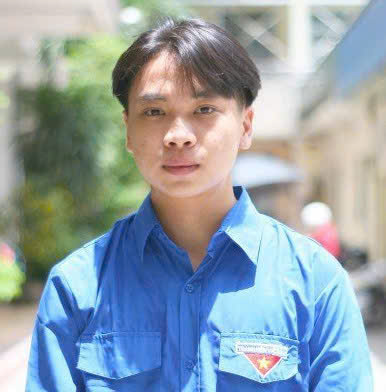
\includegraphics[width=1in,height=1.25in,clip,keepaspectratio]{images/author/author_thong_luc.jpg}}]{Thong Luc}
Thong Luc is a final-year undergraduate student in the B.Sc. program in Computer Science with the Faculty of Information Technology, University of Science, Vietnam National University Ho Chi Minh City, Vietnam. His research interests include computer vision, deep learning, medical image analysis, image segmentation, and interactive prompt-guided segmentation. His current work focuses on prompt-guided segmentation for bone radiographic images using deep learning.
\end{IEEEbiography}

\begin{biographynophoto}{Nguyen Huu Binh}
Nguyen Huu Binh is currently an undergraduate student in Computer Science with the Faculty of Information Technology, University of Science, Vietnam National University Ho Chi Minh City, Vietnam. His research interests include computer vision, deep learning, and image segmentation. His current research focuses on deep learning methods for medical image segmentation using visual prompts.
\end{biographynophoto}

\begin{IEEEbiography}[{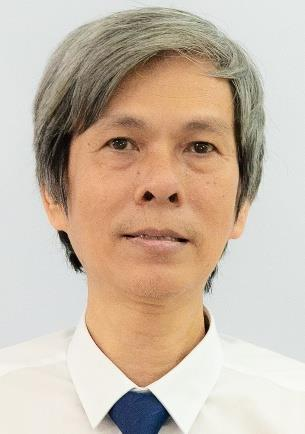
\includegraphics[width=1in,height=1.25in,clip,keepaspectratio]{images/author/author_ly_quoc_ngoc.jpg}}]{Ly Quoc Ngoc}
Ly Quoc Ngoc (Associate Professor, Ph.D.) is Head of the Department of Computer Vision and Cognitive Cybernetics, Faculty of Information Technology, University of Science, Vietnam National University Ho Chi Minh City, Vietnam. He received the B.Sc. degree in Mechanics and Mathematics, the M.Sc. degree in Computer Science, and the D.Sc. degree in Computer Science, all from the University of Science, Ho Chi Minh City, in 1987, 1996, and 2009, respectively. His research interests include artificial intelligence, machine learning, computer vision, digital image and video processing, computer graphics, multivariate statistical analysis, and medical image analysis. He has authored or co-authored nearly 70 papers in conference proceedings and academic journals, and has served as principal investigator of several research projects in intelligent vision systems.
\end{IEEEbiography}


\EOD
\end{document}
